% =============================================================================
% ASTROMANAGER v1.3.0 — MANUEL UTILISATEUR (FRANÇAIS)
% =============================================================================
% Compile with: pdflatex USER_MANUAL_FR.tex (2 passes for TOC)
% =============================================================================

\documentclass[a4paper,11pt]{article}

% ── Encoding & Language ──
\usepackage[utf8]{inputenc}
\usepackage[T1]{fontenc}
\usepackage[french]{babel}

% ── Page Layout ──
\usepackage[top=2.5cm, bottom=2.5cm, left=2.5cm, right=2.5cm, headheight=22pt]{geometry}

% ── Colors ──
\usepackage[table]{xcolor}
\definecolor{mainblue}{HTML}{1a3a5c}
\definecolor{accentcyan}{HTML}{94b8c8}
\definecolor{warnorange}{HTML}{c0b098}
\definecolor{bgdark}{HTML}{0a0e1a}
\definecolor{bgmedium}{HTML}{141828}
\definecolor{successgreen}{HTML}{88b098}
\definecolor{errorcoral}{HTML}{b89090}
\definecolor{infogrey}{HTML}{90a8b8}
\definecolor{textprimary}{HTML}{c8ccd4}
\definecolor{tablegray}{HTML}{EAF0F6}
\definecolor{tablealt}{HTML}{F5F8FB}
\definecolor{linkblue}{HTML}{2a6496}
\definecolor{titlegold}{HTML}{c8a86e}

% ── Typography ──
\usepackage{lmodern}
\usepackage{microtype}
\usepackage{parskip}
\setlength{\parskip}{0.6em}

% ── Tables ──
\usepackage{booktabs}
\usepackage{colortbl}
\usepackage{tabularx}
\usepackage{longtable}
\usepackage{array}
\newcolumntype{L}[1]{>{\raggedright\arraybackslash}p{#1}}
\newcolumntype{C}[1]{>{\centering\arraybackslash}p{#1}}

% ── Lists ──
\usepackage{enumitem}
\setlist[itemize]{nosep, leftmargin=1.5em}
\setlist[enumerate]{nosep, leftmargin=1.5em}

% ── Graphics ──
\usepackage{graphicx}
\usepackage{float}

% ── Boxes (tcolorbox) ──
\usepackage[most]{tcolorbox}

\newtcolorbox{tipbox}[1][]{%
    enhanced, breakable,
    colback=mainblue!5, colframe=mainblue!70,
    coltitle=white, fonttitle=\bfseries,
    title={\raisebox{-0.1em}{\large\textbullet}~Conseil},
    left=6pt, right=6pt, top=4pt, bottom=4pt,
    arc=3pt, boxrule=0.8pt,
    #1
}

\newtcolorbox{warningbox}[1][]{%
    enhanced, breakable,
    colback=warnorange!8, colframe=warnorange!80,
    coltitle=white, fonttitle=\bfseries,
    title={\raisebox{-0.1em}{\large$\triangle$}~Attention},
    left=6pt, right=6pt, top=4pt, bottom=4pt,
    arc=3pt, boxrule=0.8pt,
    #1
}

\newtcolorbox{notebox}[1][]{%
    enhanced, breakable,
    colback=accentcyan!8, colframe=accentcyan!60,
    coltitle=white, fonttitle=\bfseries,
    title={\raisebox{-0.1em}{\large$\circ$}~Note},
    left=6pt, right=6pt, top=4pt, bottom=4pt,
    arc=3pt, boxrule=0.8pt,
    #1
}

\newtcolorbox{criticalbox}[1][]{%
    enhanced, breakable,
    colback=errorcoral!8, colframe=errorcoral!80,
    coltitle=white, fonttitle=\bfseries,
    title={\raisebox{-0.1em}{\large$\times$}~Critique},
    left=6pt, right=6pt, top=4pt, bottom=4pt,
    arc=3pt, boxrule=0.8pt,
    #1
}

\newtcolorbox{newfeaturebox}[1][]{%
    enhanced, breakable,
    colback=successgreen!8, colframe=successgreen!60,
    coltitle=white, fonttitle=\bfseries,
    title={\raisebox{-0.1em}{\large$\star$}~Nouveau dans v1.3.0},
    left=6pt, right=6pt, top=4pt, bottom=4pt,
    arc=3pt, boxrule=0.8pt,
    #1
}

% ── Headers / Footers ──
\usepackage{fancyhdr}
\pagestyle{fancy}
\fancyhf{}
\fancyhead[L]{\small\textcolor{mainblue}{\textbf{AstroManager v1.3.0}} --- Manuel Utilisateur}
\fancyhead[R]{\small\textcolor{mainblue}{\thepage}}
\fancyfoot[C]{\small\textcolor{gray}{AstroManager --- Gestion Professionnelle de Fichiers d'Astrophotographie}}
\renewcommand{\headrulewidth}{0.5pt}
\renewcommand{\footrulewidth}{0.3pt}
\renewcommand{\headrule}{\hbox to\headwidth{\color{mainblue}\leaders\hrule height \headrulewidth\hfill}}
\renewcommand{\footrule}{\hbox to\headwidth{\color{gray!50}\leaders\hrule height \footrulewidth\hfill}}

% ── Hyperlinks ──
\usepackage[colorlinks=true, linkcolor=mainblue, urlcolor=linkblue, citecolor=mainblue, bookmarks=true, pdfauthor={ARP273-ROSE}, pdftitle={AstroManager}]{hyperref}

% ── Section styling ──
\usepackage{titlesec}
\titleformat{\section}
    {\normalfont\Large\bfseries\color{mainblue}}{\thesection}{1em}{}[\vspace{-0.3em}\textcolor{mainblue!30}{\rule{\textwidth}{0.4pt}}]
\titleformat{\subsection}
    {\normalfont\large\bfseries\color{mainblue!85}}{\thesubsection}{0.8em}{}
\titleformat{\subsubsection}
    {\normalfont\normalsize\bfseries\color{mainblue!70}}{\thesubsubsection}{0.6em}{}

% ── Code listings ──
\usepackage{listings}
\lstset{
    basicstyle=\small\ttfamily,
    backgroundcolor=\color{tablegray},
    frame=single,
    rulecolor=\color{mainblue!30},
    breaklines=true,
    showstringspaces=false,
    keywordstyle=\color{mainblue}\bfseries,
    stringstyle=\color{successgreen!80!black},
    commentstyle=\color{gray}\itshape,
    xleftmargin=1em,
    framexleftmargin=0.5em,
}

% ── Miscellaneous ──
\usepackage{pifont}
\newcommand{\cmark}{\ding{51}}
\newcommand{\xmark}{\ding{55}}

% ── Prevent widows/orphans ──
\widowpenalty=10000
\clubpenalty=10000


% =============================================================================
% DOCUMENT BEGIN
% =============================================================================

% ===================================================================
% Format maison des PDF (14/10/2026) : titres sans-serif colorés (sky,
% alert), en-tête et pied sobres, anti-titres orphelins, captures réelles.
% Les noms de couleurs historiques sont ramenés à la palette maison.
% ===================================================================
\usepackage{needspace}
\usepackage{listings}
\usepackage{tabularx}
\usepackage{booktabs}
\usepackage{etoolbox}
\usepackage{fontawesome5}
\input{version}
\definecolor{sky}{HTML}{1C6DB4}
\definecolor{skyl}{HTML}{E6F0F9}
\definecolor{alert}{HTML}{B5382B}
\definecolor{steppe}{HTML}{C08A2E}
\definecolor{summit}{HTML}{6B7A8F}
\definecolor{night}{HTML}{232A56}
\definecolor{forest}{HTML}{2E7D5B}
\definecolor{ink}{HTML}{1F2430}
\definecolor{mainblue}{HTML}{1C6DB4}
\definecolor{accentcyan}{HTML}{6B7A8F}
\definecolor{warnorange}{HTML}{C08A2E}
\definecolor{successgreen}{HTML}{2E7D5B}
\definecolor{errorcoral}{HTML}{B5382B}
\definecolor{infogrey}{HTML}{6B7A8F}
\definecolor{titlegold}{HTML}{C08A2E}
\definecolor{linkblue}{HTML}{1C6DB4}
\definecolor{tablegray}{HTML}{E6F0F9}
\definecolor{tablealt}{HTML}{F5F8FB}
\AtBeginDocument{\color{ink}}
\titleformat{\section}
  {\Large\bfseries\sffamily\color{sky}}
  {\thesection}{0.6em}{}
  [{\vspace{1pt}\color{sky!35}\titlerule[1.3pt]}]
\titlespacing*{\section}{0pt}{16pt}{8pt}
\titleformat{\subsection}{\large\bfseries\sffamily\color{alert}}{\thesubsection}{0.5em}{}
\titlespacing*{\subsection}{0pt}{12pt}{4pt}
\titleformat{\subsubsection}{\normalsize\bfseries\sffamily\color{night}}{\thesubsubsection}{0.5em}{}
\pretocmd{\section}{\needspace{12\baselineskip}}{}{}
\pretocmd{\subsection}{\needspace{6\baselineskip}}{}{}
\pretocmd{\subsubsection}{\needspace{5\baselineskip}}{}{}
\raggedbottom
\setlength{\emergencystretch}{3em}
\fancyhf{}
\renewcommand{\headrulewidth}{0.4pt}
\renewcommand{\footrulewidth}{0pt}
\renewcommand{\headrule}{\hbox to\headwidth{\color{sky!40}\leaders\hrule height \headrulewidth\hfill}}
\fancyhead[L]{\sffamily\small\color{sky}\textbf{AstroManager} \color{summit}\textbar{} Manuel d'utilisation}
\fancyhead[R]{\sffamily\small\color{summit}\thepage}
\fancyfoot[C]{\sffamily\scriptsize\color{summit}Version \VERSIONAPP{} \textbar{} github.com/ARP273-ROSE/astromanager}
\graphicspath{{../captures/}{../../assets/}}
\newcommand{\capture}[2][0.92]{\par\needspace{16\baselineskip}\begin{center}\setlength{\fboxsep}{0pt}\setlength{\fboxrule}{0.6pt}%
  \fcolorbox{summit!50}{white}{\includegraphics[width=\dimexpr#1\linewidth-1.3pt\relax]{#2}}\end{center}}
\newcommand{\menu}[1]{\textsf{\textbf{\textcolor{sky}{#1}}}}

\begin{document}

% ─────────────────────────────────────────────────────────────────────────────
% TITLE PAGE
% ─────────────────────────────────────────────────────────────────────────────
\begin{titlepage}
\thispagestyle{empty}
\vspace*{1.4cm}
\begin{center}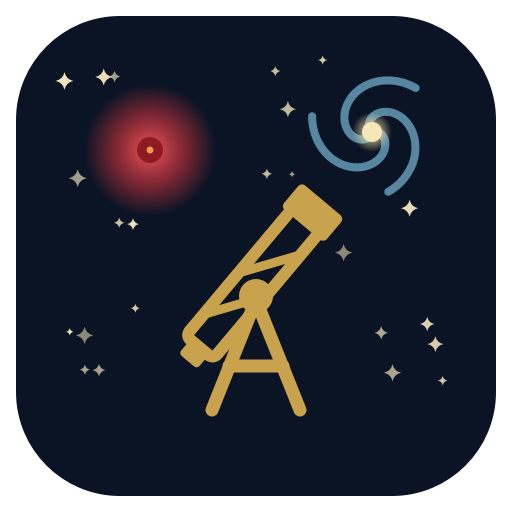
\includegraphics[width=4.6cm]{icon_512.png}\end{center}
\vspace{8mm}
{\sffamily\color{summit}\large AstroManager\par}
\vspace{4mm}
{\color{sky!35}\hrule height 2pt}
\vspace{7mm}
{\sffamily\bfseries\color{sky}\fontsize{26}{30}\selectfont Manuel d'utilisation\par}
\vspace{4mm}
{\sffamily\color{night}\large Gestion et analyse des fichiers d'astrophotographie\par}
\vspace{7mm}
{\color{sky!35}\hrule height 2pt}
\vspace{5mm}
{\sffamily\color{summit}\normalsize Version \VERSIONAPP\par}
\vfill
{\sffamily\small\color{summit} MIT \textbar{} github.com/ARP273-ROSE/astromanager\par}
\end{titlepage}

% ─────────────────────────────────────────────────────────────────────────────
% TABLE OF CONTENTS
% ─────────────────────────────────────────────────────────────────────────────
\newpage
\tableofcontents
\newpage


% =============================================================================
% 1. INTRODUCTION
% =============================================================================
\section{Introduction}
\label{sec:introduction}

\subsection{Qu'est-ce qu'AstroManager\,?}

AstroManager est une suite logicielle professionnelle d\'{e}di\'{e}e \`{a} la gestion compl\`{e}te des fichiers d'astrophotographie. Con\c{c}u pour g\'{e}rer des collections de plusieurs centaines de milliers de fichiers, il offre 18 onglets sp\'{e}cialis\'{e}s couvrant l'ensemble du workflow, de l'importation depuis l'ASIAIR jusqu'\`{a} l'exportation vers PixInsight WBPP.

\begin{tipbox}
AstroManager est capable de g\'{e}rer efficacement \textbf{plus de 200\,000 fichiers} gr\^{a}ce \`{a} son architecture multi-thread et son cache intelligent.
\end{tipbox}

\subsection{Formats support\'{e}s}

\begin{center}
\rowcolors{2}{tablealt}{white}
\begin{tabularx}{0.85\textwidth}{l X}
\toprule
\textbf{Format} & \textbf{Description} \\
\midrule
\texttt{.fits} / \texttt{.fit} / \texttt{.fts} & FITS (Flexible Image Transport System) --- standard astronomique universel \\
\texttt{.xisf} & XISF (Extensible Image Serialization Format) --- format natif PixInsight \\
\texttt{.fits.fz} / \texttt{.fz} & FITS compress\'{e} (fpack/Rice) --- compression sans perte via tuiles \\
\bottomrule
\end{tabularx}
\end{center}

\subsection{Fonctionnalit\'{e}s principales}

\begin{itemize}
    \item \textbf{Analyse universelle} --- scan r\'{e}cursif, r\'{e}solution SIMBAD, plate solving, m\'{e}t\'{e}o historique
    \item \textbf{Compression multi-codec} --- zlib, zstd, lz4 \`{a} tous les niveaux, compatible PixInsight
    \item \textbf{Import ASIAIR} --- importation, correction des headers, renommage automatique
    \item \textbf{\'{E}dition de headers} --- modification en masse avec compatibilit\'{e} N.I.N.A.
    \item \textbf{Gestion des flats} --- regroupement, couverture, suivi des master flats
    \item \textbf{Analyse qualit\'{e}} --- d\'{e}tection d'\'{e}toiles, PSF Moffat/Gaussienne, scoring 0--100
    \item \textbf{Export WBPP} --- pr\'{e}paration de l'arborescence PixInsight avec matching calibration
    \item \textbf{Suivi de cibles} --- timeline, statistiques, pr\'{e}visions m\'{e}t\'{e}o, visibilit\'{e}
    \item \textbf{Carte du ciel} --- projection Aitoff/Mollweide avec Voie Lact\'{e}e
    \item \textbf{Calendrier} --- grille mensuelle et heatmap annuelle des sessions
    \item \textbf{Analyse PixInsight} --- parsing des logs WBPP/FBP
    \item \textbf{Analyse monture} --- logs 10Micron, qualit\'{e} de suivi, FFT
    \item \textbf{Historique} --- dashboard, classements, export/import
    \item \textbf{Base de donn\'{e}es} --- cam\'{e}ras, t\'{e}lescopes, filtres, cibles
    \item \textbf{Espace disque} --- analyse stockage, doublons, organisation
    \item \textbf{Analytique N.I.N.A.} --- analyse de corr\'{e}lation et suivi d'efficacit\'{e} d'imagerie
    \item \textbf{Visionneuse d'images} --- visualisation FITS/XISF avec carte FWHM, inspecteur de coins, autostretch STF
    \item \textbf{Coupe transversale} --- comparaison de profils d'intensit\'{e} avec analyse d'att\'{e}nuation de filtre et alignement auto
\end{itemize}

\subsection{Nouveaut\'{e}s de la version 1.2.0}

La version 1.2.0 marque une \'{e}volution majeure d'AstroManager, inspir\'{e}e par les concepts d'Athenaeum et rustafits (Vilen Sharifov). Six nouveaux onglets ont \'{e}t\'{e} ajout\'{e}s~:

\begin{enumerate}
    \item \textbf{Analyse Qualit\'{e}} --- \'{e}valuation per-frame avec d\'{e}tection d'\'{e}toiles et scoring
    \item \textbf{Export WBPP} --- pr\'{e}paration automatis\'{e}e pour PixInsight WBPP
    \item \textbf{Carte du Ciel} --- visualisation c\'{e}leste de toutes les cibles observ\'{e}es
    \item \textbf{Calendrier} --- vue calendaire des sessions d'imagerie
    \item \textbf{PixInsight} --- analyse des logs de traitement
    \item \textbf{Monture} --- analyse des logs MountMonitor/10Micron
\end{enumerate}

\subsection{Nouveaut\'{e}s de la version 1.3.0}

\begin{newfeaturebox}
La version 1.3.0 ajoute \textbf{3 nouveaux onglets} inspir\'{e}s par les concepts de projets communautaires~:
\begin{itemize}
    \item \textbf{Astronalyze} (ricksastro) --- analytique et corr\'{e}lations de sessions N.I.N.A.
    \item \textbf{GalactiLog} (chvvkumar) --- suivi d'efficacit\'{e} d'imagerie et s\'{e}ries temporelles
    \item \textbf{AstroCrossSections} (brentmantooth) --- comparaison de coupes transversales d'images
\end{itemize}
\end{newfeaturebox}

Les trois nouveaux onglets~:

\begin{enumerate}
    \item \textbf{Analytique} --- import CSV N.I.N.A., corr\'{e}lations m\'{e}triques, efficacit\'{e} d'imagerie, s\'{e}ries temporelles, performance \'{e}quipement
    \item \textbf{Visionneuse d'Images} --- visualisation FITS/XISF avec autostretch STF, carte FWHM, inspecteur de coins, overlay \'{e}toiles
    \item \textbf{Coupe Transversale} --- double visionneuse, profils d'intensit\'{e} miroir\'{e}s, analyse d'att\'{e}nuation de filtre, alignement astrom\'{e}trique
\end{enumerate}

\subsection{Configuration requise}

\begin{center}
\rowcolors{2}{tablealt}{white}
\begin{tabularx}{0.85\textwidth}{l X}
\toprule
\textbf{Composant} & \textbf{Exigence} \\
\midrule
Python & 3.8 ou sup\'{e}rieur \\
Syst\`{e}me & Windows 10/11, Linux, macOS \\
RAM & 4~Go minimum, 8~Go recommand\'{e}s \\
Espace disque & 200~Mo (application + d\'{e}pendances) \\
PyQt6 & 6.2+ \\
Astropy & 5.0+ \\
NumPy & 1.20+ \\
Matplotlib & 3.5+ \\
\bottomrule
\end{tabularx}
\end{center}

\begin{notebox}
Des d\'{e}pendances optionnelles (zstandard, lz4, astroquery, scipy) sont install\'{e}es automatiquement au premier lancement si n\'{e}cessaire. La version 1.3.0 utilise \'{e}galement des biblioth\`{e}ques optionnelles suppl\'{e}mentaires~:
\begin{itemize}
    \item \texttt{pyqtgraph} ($\geq$0.13) --- affichage d'images acc\'{e}l\'{e}r\'{e} GPU (fallback matplotlib si absent)
    \item \texttt{photutils} ($\geq$1.5) --- d\'{e}tection d'\'{e}toiles et photom\'{e}trie pour la carte FWHM
    \item \texttt{astroalign} --- alignement astrom\'{e}trique par \'{e}toiles pour les coupes transversales
    \item \texttt{scikit-image} --- traitement d'image avanc\'{e} (segmentation, morphologie)
\end{itemize}
\end{notebox}


% =============================================================================
% 2. INSTALLATION
% =============================================================================
\section{Installation}
\label{sec:install}

\subsection{L'installeur (recommandé)}

Les paquets prêts à l'emploi, Python et toutes les dépendances compris, sont
publiés sur la page des versions :
\url{https://github.com/ARP273-ROSE/astromanager/releases/latest}. Aucun droit
d'administrateur n'est demandé : tout s'installe dans votre profil.

\begin{center}
\begin{tabularx}{\linewidth}{@{}l>{\raggedright\arraybackslash}X@{}}
\toprule
\textbf{Système} & \textbf{Fichier et premier lancement} \\
\midrule
Windows & \texttt{AstroManager-Setup.exe}. Si SmartScreen prévient que
l'installeur n'est pas signé : \emph{Informations complémentaires}, puis
\emph{Exécuter quand même} (une seule fois). \\
macOS & \texttt{AstroManager-X.Y.Z-macos-arm64.dmg} (Apple Silicon) ou
\texttt{-macos-x86\_64.dmg} (Intel) : glisser l'application dans Applications,
puis la première fois \emph{clic droit > Ouvrir}. \\
Linux & \texttt{AstroManager-X.Y.Z-linux-x86\_64.tar.gz} (ou \texttt{-linux-arm64}) :
décompresser, puis lancer \texttt{./installer.sh} (installation dans
\texttt{\textasciitilde/.local/share}, entrée de menu, sans sudo). \\
\bottomrule
\end{tabularx}
\end{center}

Cette adresse pointe toujours vers le dernier installeur Windows :
\begin{center}\footnotesize\url{https://github.com/ARP273-ROSE/astromanager/releases/latest/download/AstroManager-Setup.exe}\end{center}

Réglages, base de données et rapports vivent hors du dossier d'installation
(\texttt{\%APPDATA\%\textbackslash AstroManager} sous Windows,
\texttt{\textasciitilde/.astromanager} ailleurs) : ils survivent aux mises à jour.

\subsection{Mises à jour}

Une fois installé, AstroManager cherche une nouvelle version au démarrage
(réglable dans \menu{Outils > Réglages}) et sur demande
(\menu{Aide > Vérifier les mises à jour}). Il ne télécharge que la petite
archive applicative depuis GitHub (toute autre adresse est refusée), la pose et
redémarre, sous Windows, macOS et Linux. Les notes de version s'affichent dans la
langue de l'interface.

\subsection{Rapports de problème}

Au premier lancement, AstroManager demande s'il peut envoyer automatiquement un
court rapport technique en cas de plantage ou de gel (version, système, trace de
l'erreur ; aucun de vos fichiers). Ce choix se modifie dans le menu \menu{Aide},
où \menu{Signaler un problème\dots} permet aussi d'écrire un signalement.

\subsection{Depuis les sources}

Python 3.10 ou plus récent. Les lanceurs portables \texttt{launch.bat} (Windows)
et \texttt{launch.sh} (Linux, macOS) créent l'environnement virtuel et installent
les dépendances au premier lancement ; à la main :

\begin{lstlisting}
pip install -r requirements.txt
python astromanager.py            # interface
python astromanager.py --help     # analyse en ligne de commande
\end{lstlisting}

\section{Interface Utilisateur}
\label{sec:interface}

\subsection{Vue d'ensemble}

L'interface d'AstroManager s'articule autour d'une fen\^{e}tre principale divis\'{e}e en trois zones~:

\begin{enumerate}
    \item \textbf{Barre de menus} --- Fichier, Outils, Affichage, Aide
    \item \textbf{Zone d'onglets} --- 18 onglets sp\'{e}cialis\'{e}s (partie principale)
    \item \textbf{Console + Barre de progression} --- sortie des op\'{e}rations en cours
\end{enumerate}

\begin{center}
\begin{tcolorbox}[
    enhanced, width=14cm,
    colback=bgdark!3, colframe=mainblue!40,
    arc=5pt, boxrule=0.5pt,
    halign=center
]
\textit{[Emplacement pour capture d'\'{e}cran de la fen\^{e}tre principale]}\\[0.3cm]
\small\textcolor{gray}{Ins\'{e}rer ici une capture montrant les 18 onglets, la console et la barre de progression.}
\end{tcolorbox}
\end{center}

\capture{fr-principal.png}

\subsection{Les 18 onglets}

\begin{center}
\rowcolors{2}{tablealt}{white}
\begin{tabularx}{\textwidth}{c l X}
\toprule
\textbf{N\textsuperscript{o}} & \textbf{Onglet} & \textbf{Fonction} \\
\midrule
1 & Analyse & Scan de fichiers, r\'{e}solution SIMBAD, plate solving, rapports \\
2 & Compression & Conversion multi-format, 9 profils, v\'{e}rification SHA-256 \\
3 & Import ASIAIR & Importation et correction des fichiers ASIAIR \\
4 & \'{E}diteur Headers & Modification en masse des headers FITS/XISF \\
5 & Gestion Flats & Regroupement, couverture, master flats \\
6 & Qualit\'{e} & D\'{e}tection d'\'{e}toiles, PSF, scoring 0--100 \\
7 & Export WBPP & Pr\'{e}paration PixInsight WBPP \\
8 & Suivi Cibles & Timeline, int\'{e}gration, m\'{e}t\'{e}o, visibilit\'{e} \\
9 & Carte du Ciel & Projection Aitoff/Mollweide \\
10 & Calendrier & Grille mensuelle, heatmap annuelle \\
11 & PixInsight & Analyse logs WBPP/FBP \\
12 & Monture & Logs MountMonitor, suivi, FFT \\
13 & Historique & Dashboard, classements, export/import \\
14 & Base de Donn\'{e}es & Cam\'{e}ras, t\'{e}lescopes, filtres, cibles \\
15 & Espace Disque & Analyse stockage, doublons, organisation \\
16 & Analytique & Import CSV N.I.N.A., corr\'{e}lations, efficacit\'{e} \textcolor{successgreen}{\textbf{NOUVEAU v1.3}} \\
17 & Visionneuse & FITS/XISF, carte FWHM, inspecteur coins, STF \textcolor{successgreen}{\textbf{NOUVEAU v1.3}} \\
18 & Coupe Transversale & Profils d'intensit\'{e}, att\'{e}nuation filtre, alignement \textcolor{successgreen}{\textbf{NOUVEAU v1.3}} \\
\bottomrule
\end{tabularx}
\end{center}

\subsection{Th\`{e}me cosmique sombre}

AstroManager utilise un th\`{e}me sombre personnalis\'{e} inspir\'{e} de l'espace profond~:

\begin{itemize}
    \item \textbf{Fond} --- d\'{e}grad\'{e} de bleus profonds (\texttt{\#080c16} \`{a} \texttt{\#2a3248})
    \item \textbf{Accents} --- cyan d\'{e}satur\'{e} (\texttt{\#94b8c8}), lavande, rose poudr\'{e}
    \item \textbf{Texte} --- gris clair (\texttt{\#c8ccd4}) sur fond sombre
    \item \textbf{Succ\`{e}s/Erreur} --- vert sauge / corail poudr\'{e} (couleurs subtiles)
    \item \textbf{Curseur cosmique} --- curseur personnalis\'{e} avec halo
\end{itemize}

Le th\`{e}me est appliqu\'{e} automatiquement et ne n\'{e}cessite aucune configuration.

\subsection{Interface bilingue (FR/EN)}

La langue est d\'{e}tect\'{e}e automatiquement depuis les param\`{e}tres syst\`{e}me. Vous pouvez la changer via~:

\begin{itemize}
    \item \textbf{Menu} $\rightarrow$ \textit{Affichage} $\rightarrow$ \textit{Langue} $\rightarrow$ \textit{Fran\c{c}ais} / \textit{English}
    \item Fichier de configuration \texttt{config.yaml}~: \texttt{application.language: fr}
\end{itemize}

\subsection{Console de sortie}

La console en bas de la fen\^{e}tre affiche en temps r\'{e}el les messages des op\'{e}rations en cours~: progression du scan, erreurs, r\'{e}sultats. Elle utilise une police monospace \texttt{Consolas} et un code couleur pour distinguer les niveaux de messages.

Raccourci~: \texttt{Ctrl+\`{}} pour afficher/masquer la console.

\subsection{Raccourcis clavier}

\begin{center}
\rowcolors{2}{tablealt}{white}
\begin{tabularx}{0.7\textwidth}{l X}
\toprule
\textbf{Raccourci} & \textbf{Action} \\
\midrule
\texttt{Ctrl+O} & Ouvrir un dossier \\
\texttt{Ctrl+Q} & Quitter l'application \\
\texttt{Ctrl+,} & Ouvrir les r\'{e}glages \\
\texttt{Ctrl+\`{}} & Basculer la console \\
\texttt{F1} & Afficher le guide utilisateur \\
\bottomrule
\end{tabularx}
\end{center}


% =============================================================================
% 4. ONGLET ANALYSE
% =============================================================================
\subsection{Menu Aide, manuel et apparence}

Le menu \menu{Aide} ouvre ce \textbf{manuel PDF} dans la langue de
l'interface (\menu{Manuel (PDF)}, \texttt{Maj+F1}), le guide intégré (F1), les
raccourcis, la recherche de mises à jour, \menu{Signaler un problème\dots} et la
case \menu{Envoyer automatiquement les rapports de problème}.

L'apparence est \textbf{figée} : style Fusion, palette cosmique complète et
police embarquée (Source Sans 3), identiques sur les trois systèmes et
indépendantes de leur thème clair ou sombre. Sous Linux, les boîtes
\emph{Ouvrir}, \emph{Enregistrer} et \emph{Choisir un dossier} sont
l'explorateur complet de Qt (barre latérale avec dossier personnel, Bureau,
Documents, supports montés), et non la boîte réduite du portail du bureau.

\section{Analyse}
\label{sec:analyse}

L'onglet \textbf{Analyse} est le c\oe{}ur d'AstroManager. Il permet de scanner r\'{e}cursivement un dossier contenant des fichiers astronomiques et de g\'{e}n\'{e}rer un rapport complet.

\subsection{S\'{e}lection du dossier}

\begin{enumerate}
    \item Cliquer sur \textbf{Parcourir} pour choisir le dossier contenant vos fichiers FITS/XISF
    \item Le chemin s'affiche dans la barre de saisie (modifiable manuellement)
    \item L'analyse est r\'{e}cursive~: tous les sous-dossiers sont inclus
\end{enumerate}

\begin{notebox}
Les dossiers suivants sont automatiquement exclus du scan~: \texttt{extracted\_*}, \texttt{duplicates\_*}, \texttt{fits\_originals\_*}, \texttt{*\_fits\_fz\_backup}.
\end{notebox}

\subsection{Options d'analyse}

\begin{itemize}
    \item \textbf{R\'{e}solution SIMBAD} --- interroge le service CDS SIMBAD pour identifier les objets astronomiques \`{a} partir du champ \texttt{OBJECT} dans les headers
    \item \textbf{Plate Solving} --- r\'{e}solution astrom\'{e}trique via ASTAP ou Astrometry.net pour d\'{e}terminer les coordonn\'{e}es c\'{e}lestes exactes et d\'{e}tecter les r\'{e}ducteurs de focale
    \item \textbf{M\'{e}t\'{e}o historique} --- r\'{e}cup\`{e}re les donn\'{e}es m\'{e}t\'{e}o (couverture nuageuse, temp\'{e}rature, humidit\'{e}, seeing) via l'API Open-Meteo pour chaque date d'observation
    \item \textbf{Plate solving par lot} --- r\'{e}sout automatiquement tous les LIGHT bruts non-r\'{e}solus (FITS/XISF/FITS.FZ), \'{e}crit les WCS dans les headers
\end{itemize}

\subsection{R\'{e}sultats et rapports}

Apr\`{e}s l'analyse, AstroManager g\'{e}n\`{e}re~:

\begin{itemize}
    \item Un \textbf{r\'{e}sum\'{e}} dans la console (nombre de fichiers, types, cibles d\'{e}tect\'{e}es)
    \item Un \textbf{tableau d\'{e}taill\'{e}} avec les informations de chaque fichier
    \item Un \textbf{rapport CSV} exportable contenant toutes les m\'{e}tadonn\'{e}es
    \item Les donn\'{e}es sont automatiquement enregistr\'{e}es dans la base de donn\'{e}es locale
\end{itemize}

\subsection{D\'{e}tection des doublons}

AstroManager d\'{e}tecte les doublons \`{a} deux niveaux~:

\begin{enumerate}
    \item \textbf{Par nom} --- fichiers avec le m\^{e}me nom de base mais diff\'{e}rentes extensions (.fits, .xisf, .fits.fz)
    \item \textbf{Par contenu} --- fichiers avec la m\^{e}me signature (DATE-OBS, type, exposition, dimensions, binning, filtre, objet, instrument, t\'{e}lescope)
\end{enumerate}

\begin{warningbox}
La d\'{e}tection par contenu n\'{e}cessite un champ \texttt{DATE-OBS} valide. Les fichiers sans horodatage sont trait\'{e}s comme uniques pour \'{e}viter les faux positifs.
\end{warningbox}


% =============================================================================
% 5. ONGLET COMPRESSION
% =============================================================================
\section{Compression}
\label{sec:compression}

L'onglet \textbf{Compression} permet de convertir vos fichiers entre tous les formats support\'{e}s avec 9 profils de compression.

\capture{fr-compression.png}

\subsection{Les 9 profils de compression}

\begin{center}
\rowcolors{2}{tablealt}{white}
\begin{tabularx}{\textwidth}{l c c X}
\toprule
\textbf{Profil} & \textbf{Codec} & \textbf{Niveau} & \textbf{Caract\'{e}ristiques} \\
\midrule
\texttt{zlib\_1} & zlib & 1 & Rapide, compression l\'{e}g\`{e}re \\
\texttt{zlib\_6} & zlib & 6 & \'{E}quilibr\'{e} (d\'{e}faut PixInsight) \\
\texttt{zlib\_9} & zlib & 9 & Compression maximale, plus lent \\
\texttt{zstd\_3} & Zstandard & 3 & Rapide, bonne compression \\
\texttt{zstd\_6} & Zstandard & 6 & \'{E}quilibr\'{e} \\
\texttt{zstd\_10} & Zstandard & 10 & Bonne compression \\
\texttt{zstd\_19} & Zstandard & 19 & Compression maximale Zstd \\
\texttt{lz4} & LZ4 & --- & Tr\`{e}s rapide, compression mod\'{e}r\'{e}e \\
\texttt{lz4\_hc} & LZ4 HC & --- & Plus lent que LZ4, meilleure compression \\
\bottomrule
\end{tabularx}
\end{center}

\begin{tipbox}
Pour un usage quotidien, \texttt{zstd\_3} offre le meilleur compromis vitesse/compression. Pour l'archivage long terme, pr\'{e}f\'{e}rez \texttt{zstd\_19} ou \texttt{zlib\_9}.
\end{tipbox}

\subsection{Conversions support\'{e}es}

Toutes les combinaisons sont possibles~:

\begin{center}
\begin{tabular}{lccc}
\toprule
& \textbf{$\rightarrow$ XISF} & \textbf{$\rightarrow$ FITS} & \textbf{$\rightarrow$ FITS.FZ} \\
\midrule
\textbf{FITS $\rightarrow$}    & \cmark & --- & \cmark \\
\textbf{XISF $\rightarrow$}    & \cmark & \cmark & \cmark \\
\textbf{FITS.FZ $\rightarrow$} & \cmark & \cmark & --- \\
\bottomrule
\end{tabular}
\end{center}

\subsection{V\'{e}rification d'int\'{e}grit\'{e} (SHA-256)}

Apr\`{e}s chaque conversion, AstroManager calcule un hash SHA-256 des donn\'{e}es d'image pour v\'{e}rifier que la conversion est sans perte. Le hash est \'{e}galement stock\'{e} dans les m\'{e}tadonn\'{e}es du fichier de sortie.

\subsection{Traitement parall\`{e}le}

La compression utilise un \texttt{ProcessPoolExecutor} adapt\'{e} au nombre de c\oe{}urs CPU d\'{e}tect\'{e}s. Le nombre de workers est configurable dans les r\'{e}glages.

\begin{notebox}
Les codecs Zstandard et LZ4 n\'{e}cessitent les packages Python \texttt{zstandard} et \texttt{lz4}. Ils sont install\'{e}s automatiquement au premier lancement.
\end{notebox}


% =============================================================================
% 6. ONGLET IMPORT ASIAIR
% =============================================================================
\section{Import ASIAIR}
\label{sec:asiair}

L'onglet \textbf{Import ASIAIR} permet d'importer et de corriger les fichiers g\'{e}n\'{e}r\'{e}s par la ZWO ASIAIR (Mini, Plus, Pro).

\subsection{Probl\`{e}mes connus des fichiers ASIAIR}

Les fichiers FITS produits par l'ASIAIR pr\'{e}sentent plusieurs particularit\'{e}s~:

\begin{itemize}
    \item \textbf{BZERO/BSCALE} --- les cam\'{e}ras ZWO stockent les entiers non-sign\'{e}s en sign\'{e}s (standard FITS). AstroManager utilise \texttt{memmap=False} pour lire correctement ces donn\'{e}es
    \item \textbf{Headers incomplets} --- certains champs N.I.N.A. sont absents ou diff\'{e}rents
    \item \textbf{Nommage non-standard} --- les noms de fichiers ne suivent pas les conventions classiques
\end{itemize}

\subsection{Workflow d'importation}

\begin{enumerate}
    \item \textbf{S\'{e}lectionner le dossier source} --- dossier ASIAIR contenant les sous-dossiers Light, Dark, Flat, Bias
    \item \textbf{S\'{e}lectionner le dossier destination} --- o\`{u} les fichiers corrig\'{e}s seront copi\'{e}s
    \item \textbf{Configurer les corrections} --- headers \`{a} ajouter/modifier, pattern de renommage
    \item \textbf{Lancer l'import} --- copie, correction des headers et renommage automatique
\end{enumerate}

\subsection{Corrections de headers}

L'importation peut automatiquement~:

\begin{itemize}
    \item Ajouter les champs \texttt{TELESCOP}, \texttt{INSTRUME}, \texttt{FOCALLEN} s'ils sont absents
    \item Corriger le champ \texttt{IMAGETYP} pour conformit\'{e} N.I.N.A.
    \item Calculer et ajouter le champ \texttt{XBINNING}/\texttt{YBINNING}
    \item G\'{e}n\'{e}rer un nom de fichier conforme au pattern N.I.N.A. configur\'{e}
\end{itemize}

\begin{criticalbox}
Les fichiers ASIAIR avec BZERO/BSCALE ne peuvent \textbf{pas} \^{e}tre lus en mode memory-map. AstroManager g\`{e}re cela automatiquement, mais si vous utilisez d'autres outils, assurez-vous qu'ils supportent ce cas.
\end{criticalbox}


% =============================================================================
% 7. ONGLET EDITEUR HEADERS
% =============================================================================
\section{\'{E}diteur de Headers}
\label{sec:headers}

L'onglet \textbf{\'{E}diteur Headers} permet de modifier en masse les m\'{e}tadonn\'{e}es FITS/XISF de vos fichiers.

\subsection{\'{E}dition en masse}

\begin{enumerate}
    \item \textbf{S\'{e}lectionner les fichiers} --- parcourir un dossier ou glisser-d\'{e}poser
    \item \textbf{Choisir les champs} --- s\'{e}lectionner les keywords \`{a} modifier
    \item \textbf{Entrer les valeurs} --- saisir les nouvelles valeurs
    \item \textbf{Appliquer} --- les modifications sont \'{e}crites dans tous les fichiers s\'{e}lectionn\'{e}s
\end{enumerate}

\subsection{Champs courants}

\begin{center}
\rowcolors{2}{tablealt}{white}
\begin{tabularx}{\textwidth}{l l X}
\toprule
\textbf{Keyword} & \textbf{Type} & \textbf{Description} \\
\midrule
\texttt{OBJECT} & Texte & Nom de l'objet astronomique \\
\texttt{TELESCOP} & Texte & Nom du t\'{e}lescope \\
\texttt{INSTRUME} & Texte & Nom de la cam\'{e}ra \\
\texttt{FILTER} & Texte & Nom du filtre utilis\'{e} \\
\texttt{FOCALLEN} & Nombre & Focale en mm \\
\texttt{EXPTIME} & Nombre & Temps d'exposition en secondes \\
\texttt{CCD-TEMP} & Nombre & Temp\'{e}rature du capteur en \textdegree{}C \\
\texttt{GAIN} & Entier & Gain de la cam\'{e}ra \\
\texttt{OFFSET} & Entier & Offset de la cam\'{e}ra \\
\texttt{XBINNING} & Entier & Binning horizontal \\
\texttt{YBINNING} & Entier & Binning vertical \\
\texttt{IMAGETYP} & Texte & Type d'image (LIGHT, DARK, FLAT, BIAS) \\
\bottomrule
\end{tabularx}
\end{center}

\subsection{Compatibilit\'{e} N.I.N.A.}

AstroManager reconna\^{i}t les patterns de nommage N.I.N.A. et peut automatiquement~:

\begin{itemize}
    \item D\'{e}tecter le pattern utilis\'{e} dans les noms de fichiers existants
    \item Proposer un renommage automatique apr\`{e}s modification des headers
    \item G\'{e}n\'{e}rer des noms conformes au pattern configur\'{e} (ex.~: \texttt{TARGET\_FILTER\_EXP\_YYYYMMDD\_N})
\end{itemize}

\begin{tipbox}
Apr\`{e}s avoir modifi\'{e} un header (par exemple le champ \texttt{OBJECT}), AstroManager propose automatiquement de renommer le fichier pour refl\'{e}ter le changement.
\end{tipbox}

\subsection{\'{E}dition XISF}

L'\'{e}dition des headers XISF utilise le parsing XML s\'{e}curis\'{e} via \texttt{defusedxml} pour la lecture et \texttt{xml.etree.ElementTree} pour la construction d'\'{e}l\'{e}ments. Les pr\'{e}fixes d'espace de noms sont pr\'{e}serv\'{e}s pour \'{e}viter toute corruption.

\begin{warningbox}
\texttt{defusedxml} ne fournit pas de fonction \texttt{SubElement}. AstroManager utilise automatiquement la biblioth\`{e}que standard pour la cr\'{e}ation de nouveaux \'{e}l\'{e}ments XML tout en prot\'{e}geant le parsing contre les attaques XXE.
\end{warningbox}


% =============================================================================
% 8. ONGLET GESTION FLATS
% =============================================================================
\section{Gestion des Flats}
\label{sec:flats}

L'onglet \textbf{Gestion Flats} aide \`{a} organiser et suivre vos flat frames pour un traitement optimal.

\subsection{Regroupement automatique}

Les flats sont automatiquement regroup\'{e}s par~:

\begin{itemize}
    \item \textbf{Filtre} --- L, R, G, B, Ha, SII, OIII, etc.
    \item \textbf{Optique} --- t\'{e}lescope + focale + rapport f/D
    \item \textbf{Rotation} --- angle de la cam\'{e}ra
    \item \textbf{Binning} --- 1\texttimes{}1, 2\texttimes{}2, etc.
    \item \textbf{Temp\'{e}rature} --- temp\'{e}rature du capteur
\end{itemize}

\subsection{Analyse de couverture}

Pour chaque groupe, AstroManager affiche~:

\begin{itemize}
    \item Le \textbf{nombre de flats} disponibles
    \item La \textbf{date la plus r\'{e}cente} de prise de vue
    \item L'\textbf{ADU moyen} et la \textbf{r\'{e}gularit\'{e}} (uniformit\'{e} du signal)
    \item La \textbf{couverture} --- quels filtres/optiques sont couverts ou manquants
\end{itemize}

\begin{tipbox}
Visez au moins 20--30 flats par groupe pour un master flat de qualit\'{e}. AstroManager signale en orange les groupes avec moins de 15 flats et en rouge ceux avec moins de 5.
\end{tipbox}

\subsection{Suivi des Master Flats}

L'onglet permet de r\'{e}f\'{e}rencer vos master flats existants et de v\'{e}rifier qu'ils correspondent bien aux donn\'{e}es LIGHT que vous souhaitez traiter.


% =============================================================================
% 9. ONGLET ANALYSE QUALITE (NOUVEAU)
% =============================================================================
\section{Analyse Qualit\'{e}}
\label{sec:qualite}

\begin{tcolorbox}[
    enhanced, colback=successgreen!8, colframe=successgreen!60,
    coltitle=white, fonttitle=\bfseries,
    title={NOUVEAU dans v1.2.0}
]
L'onglet \textbf{Qualit\'{e}} est un ajout majeur de la version 1.2.0. Il fournit une analyse per-frame compl\`{e}te avec d\'{e}tection d'\'{e}toiles, ajustement PSF, et scoring 0--100.
\end{tcolorbox}

\capture{fr-qualite.png}

\subsection{D\'{e}tection d'\'{e}toiles}

AstroManager d\'{e}tecte automatiquement les \'{e}toiles dans chaque image en utilisant~:

\begin{itemize}
    \item Un algorithme de d\'{e}tection par seuil adaptatif (DAOFind-like)
    \item Filtrage des artefacts et des pixels chauds
    \item Catalogage des positions, intensit\'{e}s et FWHM pr\'{e}liminaires
\end{itemize}

\subsection{Ajustement PSF (Moffat \& Gaussienne)}

Pour chaque \'{e}toile d\'{e}tect\'{e}e, deux mod\`{e}les de PSF (Point Spread Function) sont ajust\'{e}s~:

\begin{itemize}
    \item \textbf{Mod\`{e}le de Moffat} --- $I(r) = I_0 \left(1 + \left(\frac{r}{\alpha}\right)^2\right)^{-\beta}$, plus r\'{e}aliste pour les \'{e}toiles astronomiques
    \item \textbf{Mod\`{e}le Gaussien} --- $I(r) = I_0 \exp\left(-\frac{r^2}{2\sigma^2}\right)$, classique et rapide
\end{itemize}

\subsection{M\'{e}triques extraites}

\begin{center}
\rowcolors{2}{tablealt}{white}
\begin{tabularx}{\textwidth}{l l X}
\toprule
\textbf{M\'{e}trique} & \textbf{Unit\'{e}} & \textbf{Description} \\
\midrule
FWHM & pixels / arcsec & Largeur \`{a} mi-hauteur de la PSF \\
HFR & pixels & Rayon de demi-flux (Half Flux Radius) \\
Excentricit\'{e} & 0--1 & D\'{e}formation elliptique des \'{e}toiles \\
SNR & ratio & Rapport signal sur bruit \\
Nombre d'\'{e}toiles & --- & \'{E}toiles d\'{e}tect\'{e}es et valides \\
Tra\^{i}n\'{e}es satellites & oui/non & D\'{e}tection de tra\^{i}n\'{e}es lin\'{e}aires (Starlink, etc.) \\
\bottomrule
\end{tabularx}
\end{center}

\subsection{Scoring 0--100}

Chaque frame re\c{c}oit un score de qualit\'{e} de 0 (inutilisable) \`{a} 100 (excellent)~:

\begin{center}
\rowcolors{2}{tablealt}{white}
\begin{tabularx}{0.8\textwidth}{c l X}
\toprule
\textbf{Score} & \textbf{Qualit\'{e}} & \textbf{Couleur} \\
\midrule
80--100 & Excellente & \textcolor{successgreen}{\rule{1cm}{8pt}} Vert sauge \\
60--79 & Bonne & \textcolor{accentcyan}{\rule{1cm}{8pt}} Cyan \\
40--59 & M\'{e}diocre & \textcolor{warnorange}{\rule{1cm}{8pt}} Beige/Tan \\
20--39 & Mauvaise & \textcolor{errorcoral}{\rule{1cm}{8pt}} Corail \\
0--19 & Inutilisable & \textcolor{errorcoral}{\rule{1cm}{8pt}} Corail gras \\
\bottomrule
\end{tabularx}
\end{center}

\subsection{Rejet de frames}

Le syst\`{e}me de scoring permet de~:

\begin{itemize}
    \item D\'{e}finir un \textbf{seuil de rejet} (ex.~: rejeter tout frame < 30)
    \item Visualiser la \textbf{distribution des scores} (histogramme)
    \item \textbf{Exporter la liste} des frames accept\'{e}s/rejet\'{e}s en CSV
    \item Identifier les frames avec \textbf{tra\^{i}n\'{e}es de satellites}
\end{itemize}

\subsection{Carte des \'{e}toiles}

La \textbf{carte des \'{e}toiles} (Star Map) affiche les positions des \'{e}toiles d\'{e}tect\'{e}es superpos\'{e}es sur l'image, avec~:

\begin{itemize}
    \item Cercles proportionnels au FWHM de chaque \'{e}toile
    \item Code couleur par qualit\'{e} (FWHM, excentricit\'{e})
    \item Grille de d\'{e}formation montrant la variation de PSF sur le champ
\end{itemize}


% =============================================================================
% 10. ONGLET EXPORT WBPP (NOUVEAU)
% =============================================================================
\section{Export WBPP}
\label{sec:wbpp}

\begin{tcolorbox}[
    enhanced, colback=successgreen!8, colframe=successgreen!60,
    coltitle=white, fonttitle=\bfseries,
    title={NOUVEAU dans v1.2.0}
]
L'onglet \textbf{Export WBPP} automatise la pr\'{e}paration de l'arborescence de fichiers pour le script Weighted Batch PreProcessing (WBPP) de PixInsight.
\end{tcolorbox}

\subsection{Principe}

WBPP attend une structure de dossiers pr\'{e}cise~:

\begin{lstlisting}[title=Structure WBPP typique]
Export_WBPP/
  Target_A/
    LIGHT/
      Ha/  (fichiers Light Ha)
      OIII/ (fichiers Light OIII)
    DARK/   (darks correspondants)
    FLAT/
      Ha/  (flats Ha)
      OIII/ (flats OIII)
    BIAS/   (bias correspondants)
  Target_B/
    ...
\end{lstlisting}

\subsection{Templates}

Les templates d\'{e}finissent la structure de dossiers g\'{e}n\'{e}r\'{e}e. Vous pouvez utiliser les templates par d\'{e}faut ou cr\'{e}er les v\^{o}tres.

\subsection{Matching de calibration}

Le matching de calibration est le c\oe{}ur de l'Export WBPP. Il associe automatiquement les frames de calibration (Dark, Flat, Bias) aux frames Light en fonction de \textbf{8 param\`{e}tres}~:

\begin{center}
\rowcolors{2}{tablealt}{white}
\begin{tabularx}{\textwidth}{c l X}
\toprule
\textbf{N\textsuperscript{o}} & \textbf{Param\`{e}tre} & \textbf{Description} \\
\midrule
1 & Cam\'{e}ra & M\^{e}me capteur (INSTRUME) \\
2 & Binning & M\^{e}me facteur de binning \\
3 & Gain & M\^{e}me gain (ou plage acceptable) \\
4 & Offset & M\^{e}me offset \\
5 & Temp\'{e}rature & Temp\'{e}rature capteur (tol\'{e}rance configurable) \\
6 & Exposition & M\^{e}me dur\'{e}e (pour les darks) \\
7 & Filtre & M\^{e}me filtre (pour les flats) \\
8 & Optique & M\^{e}me t\'{e}lescope/focale (pour les flats) \\
\bottomrule
\end{tabularx}
\end{center}

\subsubsection{Les 3 modes de matching}

\begin{enumerate}
    \item \textbf{Strict} --- tous les param\`{e}tres doivent correspondre exactement
    \item \textbf{Normal} --- tol\'{e}rances sur la temp\'{e}rature ($\pm$2\textdegree{}C) et l'exposition ($\pm$5\%)
    \item \textbf{Souple} --- tol\'{e}rances \'{e}largies, matching partiel accept\'{e}
\end{enumerate}

\subsubsection{Cha\^{i}nes de fallback}

Si aucun match exact n'est trouv\'{e}, le syst\`{e}me tente des approximations successives~:

\begin{enumerate}
    \item Match exact $\rightarrow$ 2. Tol\'{e}rance temp\'{e}rature $\rightarrow$ 3. Tol\'{e}rance exposition $\rightarrow$ 4. Ignorer temp\'{e}rature
\end{enumerate}

\subsection{Score de matching (0--1)}

Chaque association re\c{c}oit un score de confiance entre 0 et 1~:

\begin{itemize}
    \item \textbf{1.0} --- match parfait sur tous les param\`{e}tres
    \item \textbf{0.8--0.99} --- petites diff\'{e}rences (temp\'{e}rature proche)
    \item \textbf{0.5--0.79} --- match acceptable avec compromis
    \item \textbf{< 0.5} --- match faible, v\'{e}rification recommand\'{e}e
\end{itemize}

\subsection{Pr\'{e}visualisation de l'arborescence}

Avant l'exportation, un \textbf{arbre de pr\'{e}visualisation} montre la structure qui sera cr\'{e}\'{e}e, avec~:

\begin{itemize}
    \item Nombre de fichiers par dossier
    \item Score de matching pour chaque association de calibration
    \item Signalement des calibrations manquantes
\end{itemize}

\subsection{Modes d'exportation}

\begin{center}
\rowcolors{2}{tablealt}{white}
\begin{tabularx}{\textwidth}{l X}
\toprule
\textbf{Mode} & \textbf{Description} \\
\midrule
\textbf{Copie} & Copie physique des fichiers (s\^{u}r, mais consomme de l'espace) \\
\textbf{Lien symbolique} & Cr\'{e}e des symlinks (rapide, \'{e}conomise l'espace, n\'{e}cessite privil\`{e}ges) \\
\textbf{Liste} & G\'{e}n\`{e}re uniquement un fichier texte avec les chemins (pour import manuel) \\
\bottomrule
\end{tabularx}
\end{center}

\begin{warningbox}
Le mode \textbf{Lien symbolique} sous Windows n\'{e}cessite les droits administrateur ou le mode d\'{e}veloppeur activ\'{e} (Windows 10 1703+). Sous Linux/macOS, aucune restriction.
\end{warningbox}


% =============================================================================
% 11. ONGLET SUIVI CIBLES
% =============================================================================
\section{Suivi de Cibles}
\label{sec:cibles}

L'onglet \textbf{Suivi Cibles} offre une vue compl\`{e}te de votre progression sur chaque cible astronomique.

\subsection{Timeline}

La timeline affiche chronologiquement toutes les sessions d'imagerie pour chaque cible~:

\begin{itemize}
    \item \textbf{Dates} d'observation
    \item \textbf{Dur\'{e}e} de chaque session
    \item \textbf{Filtres} utilis\'{e}s et temps d'int\'{e}gration par filtre
    \item \textbf{Conditions} (seeing, couverture nuageuse si disponibles)
\end{itemize}

\subsection{Statistiques d'int\'{e}gration}

Pour chaque cible, AstroManager calcule~:

\begin{itemize}
    \item \textbf{Temps total d'int\'{e}gration} --- somme de toutes les expositions valides
    \item \textbf{R\'{e}partition par filtre} --- L, R, G, B, Ha, SII, OIII avec temps et nombre de subs
    \item \textbf{Qualit\'{e} moyenne} --- FWHM moyen, excentricit\'{e} moyenne (si analyse qualit\'{e} effectu\'{e}e)
    \item \textbf{Progression} --- objectif d'int\'{e}gration vs r\'{e}alis\'{e}
\end{itemize}

\subsection{Pr\'{e}visions m\'{e}t\'{e}o}

L'int\'{e}gration avec l'API Open-Meteo fournit~:

\begin{itemize}
    \item \textbf{M\'{e}t\'{e}o des prochains jours} --- couverture nuageuse, temp\'{e}rature, humidit\'{e}
    \item \textbf{Recommandation} --- nuits favorables pour imager
    \item \textbf{Historique} --- conditions pass\'{e}es pour chaque session enregistr\'{e}e
\end{itemize}

\subsection{Visibilit\'{e}}

Pour chaque cible, calcul de~:

\begin{itemize}
    \item \textbf{Hauteur maximale} au-dessus de l'horizon pour la nuit en cours
    \item \textbf{Fen\^{e}tre de visibilit\'{e}} --- heures de d\'{e}but et fin optimales
    \item \textbf{Saison optimale} --- mois de l'ann\'{e}e avec la meilleure visibilit\'{e}
\end{itemize}


% =============================================================================
% 12. ONGLET CARTE DU CIEL (NOUVEAU)
% =============================================================================
\section{Carte du Ciel}
\label{sec:carteciel}

\begin{tcolorbox}[
    enhanced, colback=successgreen!8, colframe=successgreen!60,
    coltitle=white, fonttitle=\bfseries,
    title={NOUVEAU dans v1.2.0}
]
L'onglet \textbf{Carte du Ciel} affiche une carte c\'{e}leste interactive montrant toutes vos cibles observ\'{e}es.
\end{tcolorbox}

\capture{fr-ciel.png}

\subsection{Projections disponibles}

\begin{itemize}
    \item \textbf{Aitoff} --- projection pseudo-azimutale \'{e}gale en surface, classique en astronomie
    \item \textbf{Mollweide} --- projection \'{e}gale en surface, bords plus arrondis
\end{itemize}

\subsection{Codage couleur}

Les cibles sont affich\'{e}es avec un codage couleur configurable~:

\subsubsection{Par type d'objet}

\begin{center}
\rowcolors{2}{tablealt}{white}
\begin{tabularx}{0.85\textwidth}{l l X}
\toprule
\textbf{Type} & \textbf{Couleur} & \textbf{Exemples} \\
\midrule
Galaxies & \textcolor[HTML]{b89898}{\rule{1cm}{8pt}} Rose poudr\'{e} & M31, NGC 891, Arp 273 \\
N\'{e}buleuses \'{e}mission/HII & \textcolor[HTML]{90b098}{\rule{1cm}{8pt}} Vert doux & M42, IC 1805, NGC 7000 \\
N\'{e}buleuses plan\'{e}taires & \textcolor[HTML]{a8a0c0}{\rule{1cm}{8pt}} Lavande & M57, NGC 7293 \\
N\'{e}buleuses r\'{e}flexion & \textcolor[HTML]{90a0b8}{\rule{1cm}{8pt}} Bleu gris & M78, IC 2118 \\
Amas ouverts & \textcolor[HTML]{b8b090}{\rule{1cm}{8pt}} Bl\'{e} & M45, NGC 869 \\
Amas globulaires & \textcolor[HTML]{c0a898}{\rule{1cm}{8pt}} Saumon & M13, NGC 5139 \\
\bottomrule
\end{tabularx}
\end{center}

\subsubsection{Par filtre}

Les filtres utilisent la palette de couleurs d\'{e}finie dans le th\`{e}me (L=blanc, R=rouge, G=vert, B=bleu, Ha=rose, SII=orange, OIII=cyan).

\subsubsection{Par temps d'int\'{e}gration}

La taille des marqueurs est proportionnelle au temps d'int\'{e}gration total. Les cibles avec plus de donn\'{e}es apparaissent plus grandes.

\subsection{Voie Lact\'{e}e}

Un contour de la Voie Lact\'{e}e peut \^{e}tre superpos\'{e} \`{a} la carte pour visualiser la bande galactique et planifier vos observations en cons\'{e}quence.

\subsection{Interactivit\'{e}}

\begin{itemize}
    \item \textbf{Tooltips} --- survoler une cible pour voir son nom, type, RA/Dec et temps d'int\'{e}gration
    \item \textbf{Grille de coordonn\'{e}es} --- RA/Dec avec labels
    \item \textbf{Zoom et d\'{e}placement} --- navigation matplotlib standard
    \item \textbf{Export} --- sauvegarde de la carte en PNG/SVG/PDF
\end{itemize}


% =============================================================================
% 13. ONGLET CALENDRIER (NOUVEAU)
% =============================================================================
\section{Calendrier}
\label{sec:calendrier}

\begin{tcolorbox}[
    enhanced, colback=successgreen!8, colframe=successgreen!60,
    coltitle=white, fonttitle=\bfseries,
    title={NOUVEAU dans v1.2.0}
]
L'onglet \textbf{Calendrier} offre une vue temporelle de votre activit\'{e} d'imagerie.
\end{tcolorbox}

\subsection{Grille mensuelle}

La grille mensuelle affiche chaque jour du mois avec~:

\begin{itemize}
    \item \textbf{Indicateur de session} --- les jours avec des donn\'{e}es sont color\'{e}s
    \item \textbf{Nombre de frames} --- affich\'{e} dans chaque case
    \item \textbf{Temps total} --- dur\'{e}e d'int\'{e}gration du jour
    \item Navigation par mois (fl\`{e}ches pr\'{e}c\'{e}dent/suivant)
\end{itemize}

\subsection{Heatmap annuelle}

La heatmap annuelle (style GitHub) montre l'ensemble de l'ann\'{e}e avec un d\'{e}grad\'{e} de couleurs~:

\begin{center}
\begin{tabular}{ccccc}
\textcolor[HTML]{0a0e1a}{\rule{0.8cm}{0.8cm}} &
\textcolor[HTML]{1a2a3a}{\rule{0.8cm}{0.8cm}} &
\textcolor[HTML]{2a4a5a}{\rule{0.8cm}{0.8cm}} &
\textcolor[HTML]{4a7a8a}{\rule{0.8cm}{0.8cm}} &
\textcolor[HTML]{94b8c8}{\rule{0.8cm}{0.8cm}} \\
\small Aucune & \small Faible & \small Moyenne & \small \'{E}lev\'{e}e & \small Tr\`{e}s \'{e}lev\'{e}e
\end{tabular}
\end{center}

\subsection{Statistiques}

Le calendrier fournit des statistiques agr\'{e}g\'{e}es~:

\begin{itemize}
    \item \textbf{Nombre de nuits} d'imagerie dans la p\'{e}riode
    \item \textbf{Temps total} d'int\'{e}gration
    \item \textbf{Moyenne par session} --- dur\'{e}e typique d'une nuit
    \item \textbf{S\'{e}rie la plus longue} --- nuits cons\'{e}cutives d'imagerie
    \item \textbf{Mois le plus productif}
\end{itemize}

\subsection{D\'{e}tails de session}

Cliquer sur un jour affiche les d\'{e}tails de la session~:

\begin{itemize}
    \item Cibles image\'{e}es
    \item Filtres utilis\'{e}s et nombre de poses
    \item Temps d'int\'{e}gration par filtre
    \item Conditions m\'{e}t\'{e}o (si disponibles)
\end{itemize}


% =============================================================================
% 14. ONGLET PIXINSIGHT (NOUVEAU)
% =============================================================================
\section{PixInsight}
\label{sec:pixinsight}

\begin{tcolorbox}[
    enhanced, colback=successgreen!8, colframe=successgreen!60,
    coltitle=white, fonttitle=\bfseries,
    title={NOUVEAU dans v1.2.0}
]
L'onglet \textbf{PixInsight} analyse les fichiers de log g\'{e}n\'{e}r\'{e}s par les scripts PixInsight.
\end{tcolorbox}

\subsection{Analyse WBPP}

Le parser WBPP (Weighted Batch PreProcessing) extrait~:

\begin{itemize}
    \item \textbf{Fichiers trait\'{e}s} --- nombre d'images par type (Light, Dark, Flat, Bias)
    \item \textbf{Calibration} --- images utilis\'{e}es et rejet\'{e}es lors de la calibration
    \item \textbf{Alignement} --- taux de succ\`{e}s, images non-align\'{e}es
    \item \textbf{Int\'{e}gration} --- poids des images dans le stack final
    \item \textbf{Pipeline} --- \'{e}tape par \'{e}tape, dur\'{e}e de chaque phase
\end{itemize}

\subsection{Analyse FBP}

Le parser FBP (Fast Batch Preprocessing) extrait des informations similaires adapt\'{e}es au workflow FBP.

\subsection{Diagnostics}

L'onglet signale automatiquement~:

\begin{itemize}
    \item Les images rejet\'{e}es et la raison du rejet
    \item Les erreurs d'alignement (star matching \'{e}chou\'{e})
    \item Les probl\`{e}mes de calibration (master manquant, mismatch)
    \item Les performances du pipeline (temps anormalement longs)
\end{itemize}


% =============================================================================
% 15. ONGLET MONTURE (NOUVEAU)
% =============================================================================
\section{Monture}
\label{sec:monture}

\begin{tcolorbox}[
    enhanced, colback=successgreen!8, colframe=successgreen!60,
    coltitle=white, fonttitle=\bfseries,
    title={NOUVEAU dans v1.2.0}
]
L'onglet \textbf{Monture} analyse les logs de suivi de votre monture, avec un support natif pour les montures 10Micron.
\end{tcolorbox}

\subsection{Analyse des logs MountMonitor}

L'onglet parse les fichiers de log g\'{e}n\'{e}r\'{e}s par MountMonitor pour~:

\begin{itemize}
    \item \textbf{Erreur de suivi} --- erreur p\'{e}riodique, erreur RMS en RA et Dec
    \item \textbf{D\'{e}rive} --- tendance de la d\'{e}rive sur une session
    \item \textbf{StDev} --- \'{e}cart-type du suivi, tol\'{e}rance configurable
    \item \textbf{V\'{e}rification post-slew} --- checkMountSettings apr\`{e}s chaque goto
\end{itemize}

\subsection{Qualit\'{e} de suivi}

Le syst\`{e}me \'{e}value la qualit\'{e} du suivi selon~:

\begin{itemize}
    \item \textbf{RMS RA} --- \'{e}cart-type en ascension droite (en arcsec)
    \item \textbf{RMS Dec} --- \'{e}cart-type en d\'{e}clinaison
    \item \textbf{P\'{e}riodicit\'{e}} --- d\'{e}tection de l'erreur p\'{e}riodique de la monture
    \item \textbf{Stabilit\'{e}} --- variation de l'erreur au cours du temps
\end{itemize}

\subsection{Analyse FFT}

La \textbf{Transform\'{e}e de Fourier Rapide} (FFT) du signal de suivi r\'{e}v\`{e}le~:

\begin{itemize}
    \item Les \textbf{fr\'{e}quences dominantes} de l'erreur p\'{e}riodique
    \item La \textbf{p\'{e}riode fondamentale} (souvent li\'{e}e \`{a} la rotation des vis sans fin)
    \item Les \textbf{harmoniques} et le \textbf{bruit} r\'{e}siduel
\end{itemize}

\begin{tipbox}
Pour les montures 10Micron (mod\'{e}lisation d'erreurs, pas d'autoguiding), le RMS de guidage sera toujours \`{a} 0. Concentrez-vous sur l'analyse FFT et la StDev du mod\`{e}le.
\end{tipbox}


% =============================================================================
% 16. ONGLET HISTORIQUE & STATISTIQUES
% =============================================================================
\section{Historique \& Statistiques}
\label{sec:historique}

L'onglet \textbf{Historique} offre un tableau de bord complet de votre activit\'{e} d'astrophotographie.

\subsection{Dashboard}

Le dashboard pr\'{e}sente en un coup d'\oe{}il~:

\begin{itemize}
    \item \textbf{Nombre total de cibles} image\'{e}es
    \item \textbf{Temps d'int\'{e}gration total} (toutes cibles, tous filtres)
    \item \textbf{Nombre de sessions} d'imagerie
    \item \textbf{Nombre de frames} enregistr\'{e}es
    \item \textbf{Volume de donn\'{e}es} analys\'{e}es
\end{itemize}

\subsection{Classements}

\begin{itemize}
    \item \textbf{Top cibles} --- cibles class\'{e}es par temps d'int\'{e}gration total
    \item \textbf{Top filtres} --- filtres les plus utilis\'{e}s
    \item \textbf{Top t\'{e}lescopes} --- instruments les plus utilis\'{e}s
    \item \textbf{Top mois} --- mois les plus productifs
\end{itemize}

\subsection{Graphiques temporels}

\begin{itemize}
    \item \textbf{\'{E}volution mensuelle} du temps d'int\'{e}gration
    \item \textbf{Nombre de sessions} par mois
    \item \textbf{Courbe de progression} cumulative
\end{itemize}

\subsection{Export / Import}

\begin{itemize}
    \item \textbf{Export JSON} --- sauvegarde compl\`{e}te de l'historique
    \item \textbf{Export CSV} --- tableau plat pour analyse dans Excel/Google Sheets
    \item \textbf{Import JSON} --- restauration ou fusion d'historiques
\end{itemize}

\begin{tipbox}
Utilisez l'export/import pour synchroniser l'historique entre plusieurs installations d'AstroManager ou pour cr\'{e}er des sauvegardes r\'{e}guli\`{e}res.
\end{tipbox}


% =============================================================================
% 17. ONGLET BASE DE DONNEES
% =============================================================================
\section{Base de Donn\'{e}es}
\label{sec:database}

L'onglet \textbf{Base de Donn\'{e}es} permet de consulter et g\'{e}rer les catalogues int\'{e}gr\'{e}s d'AstroManager.

\subsection{Cam\'{e}ras}

La base contient \textbf{1\,614 capteurs} et \textbf{2\,448 correspondances de headers}. Chaque entr\'{e}e inclut~:

\begin{itemize}
    \item Nom complet du capteur et aliases
    \item R\'{e}solution (NAXIS1 $\times$ NAXIS2)
    \item Taille de pixel (microns)
    \item Format du capteur
    \item Correspondances des keywords FITS (\texttt{INSTRUME}, \texttt{CCD-NAME}, etc.)
\end{itemize}

\subsection{T\'{e}lescopes}

La base contient \textbf{3\,991 mod\`{e}les} et \textbf{6\,605 correspondances de headers}. Chaque entr\'{e}e inclut~:

\begin{itemize}
    \item Nom du t\'{e}lescope et fabricant
    \item Focale (mm) et rapport f/D
    \item Diam\`{e}tre d'ouverture (mm)
    \item Type optique (r\'{e}fracteur, Newton, Schmidt-Cassegrain, etc.)
\end{itemize}

\subsection{Filtres}

La base contient \textbf{1\,612 filtres} et \textbf{701 aliases}. Elle g\`{e}re~:

\begin{itemize}
    \item Nom standard et aliases (ex.~: \texttt{Ha}, \texttt{H-alpha}, \texttt{656nm})
    \item Bande passante (largeur \`{a} mi-hauteur)
    \item Cat\'{e}gorie (broadband RGB, narrowband, luminance)
\end{itemize}

\subsection{Cibles}

La base contient \textbf{32\,923 objets} astronomiques couvrant~:

\begin{itemize}
    \item Catalogues~: NGC, IC, Messier, Arp, Abell, Sharpless, LBN, LDN, vdB, Barnard, Collinder, Melotte, etc.
    \item Coordonn\'{e}es (RA/Dec J2000)
    \item Type d'objet (galaxie, n\'{e}buleuse, amas, plan\'{e}taire, etc.)
    \item Noms communs et aliases
\end{itemize}


% =============================================================================
% 18. ONGLET ESPACE DISQUE
% =============================================================================
\section{Espace Disque}
\label{sec:disque}

L'onglet \textbf{Espace Disque} analyse l'utilisation du stockage de vos fichiers astronomiques.

\subsection{Analyse du stockage}

\begin{itemize}
    \item \textbf{Volume total} par format (FITS, XISF, FITS.FZ)
    \item \textbf{Volume par type} (Light, Dark, Flat, Bias)
    \item \textbf{Volume par cible}
    \item \textbf{Graphiques} --- camemberts et barres de r\'{e}partition
\end{itemize}

\subsection{D\'{e}tection de doublons}

Le syst\`{e}me de d\'{e}duplication \`{a} deux niveaux~:

\begin{enumerate}
    \item \textbf{Par nom} --- m\^{e}me fichier en .fits, .xisf et .fits.fz
    \item \textbf{Par contenu} --- signature identique (11 param\`{e}tres de header)
\end{enumerate}

\begin{itemize}
    \item Visualisation des doublons d\'{e}tect\'{e}s avec taille r\'{e}cup\'{e}rable
    \item Extraction des doublons vers un dossier d\'{e}di\'{e} (\texttt{extracted\_YYYYMMDD\_HHMMSS})
    \item Conservation du fichier dans le format pr\'{e}f\'{e}r\'{e} (XISF > FITS > FITS.FZ)
\end{itemize}

\subsection{Organisation}

L'onglet propose des presets d'organisation pour restructurer vos fichiers~:

\begin{itemize}
    \item Par \textbf{date} (\texttt{YYYY/MM/DD/})
    \item Par \textbf{cible} (\texttt{NGC7000/Ha/Light/})
    \item Par \textbf{type d'image} (\texttt{Light/Dark/Flat/Bias/})
    \item Par \textbf{t\'{e}lescope} (\texttt{Takahashi\_FC-76DCU/M31/Ha/})
\end{itemize}

\begin{warningbox}
L'organisation d\'{e}place physiquement les fichiers. Assurez-vous d'avoir une sauvegarde avant de r\'{e}organiser une grande collection. AstroManager cr\'{e}e un journal des op\'{e}rations pour permettre une annulation.
\end{warningbox}


% =============================================================================
% 19. CONFIGURATION
% =============================================================================
\section{Configuration}
\label{sec:configuration}

\subsection{Bo\^{i}te de dialogue des r\'{e}glages}

Accessible via \textbf{Outils} $\rightarrow$ \textbf{R\'{e}glages} (\texttt{Ctrl+,}), la bo\^{i}te de dialogue permet de configurer~:

\begin{center}
\rowcolors{2}{tablealt}{white}
\begin{tabularx}{\textwidth}{l l X}
\toprule
\textbf{Section} & \textbf{Param\`{e}tre} & \textbf{Description} \\
\midrule
Application & Langue & \texttt{auto}, \texttt{fr}, \texttt{en} \\
Application & Mises \`{a} jour & Intervalle de v\'{e}rification (heures) \\
Analyse & Workers & Nombre de threads pour le scan \\
Analyse & Plate solver & ASTAP ou Astrometry.net \\
Compression & Profil d\'{e}faut & Profil de compression par d\'{e}faut \\
Compression & Workers & Nombre de processus parall\`{e}les \\
WBPP & Tol\'{e}rance temp. & Tol\'{e}rance de temp\'{e}rature (\textdegree{}C) \\
WBPP & Mode matching & Strict, Normal, Souple \\
M\'{e}t\'{e}o & Coordonn\'{e}es & Latitude/Longitude du site d'observation \\
\bottomrule
\end{tabularx}
\end{center}

\subsection{Fichier \texttt{config.yaml}}

La configuration est stock\'{e}e dans un fichier YAML dans le dossier du projet~:

\begin{lstlisting}[title=Exemple de config.yaml]
application:
  language: auto
  update_check_interval_hours: 24
analysis:
  workers: 8
  plate_solver: astap
  simbad_enabled: true
compression:
  default_profile: zstd_3
  workers: 4
weather:
  latitude: 48.8566
  longitude: 2.3522
\end{lstlisting}

\begin{notebox}
Le \texttt{ConfigManager} est un singleton thread-safe. Les modifications via l'interface sont imm\'{e}diatement persist\'{e}es dans le fichier YAML.
\end{notebox}


% =============================================================================
% 20. BASE DE DONNEES SQLITE
% =============================================================================
\section{Base de Donn\'{e}es SQLite}
\label{sec:sqlite}

AstroManager utilise une base de donn\'{e}es SQLite locale pour stocker l'historique, le cache et les m\'{e}tadonn\'{e}es.

\subsection{Emplacement}

La base de donn\'{e}es \texttt{astromanager.db} est stock\'{e}e dans le \textbf{dossier du projet} (c\^{o}t\'{e} code source), pas dans \texttt{\%APPDATA\%} ni \texttt{\textasciitilde/}. Cela garantit que les donn\'{e}es suivent le projet quand il est synchronis\'{e} via NAS.

\subsection{Sch\'{e}ma v5}

Le sch\'{e}ma de la base de donn\'{e}es en version 5 comprend~:

\begin{center}
\rowcolors{2}{tablealt}{white}
\begin{tabularx}{\textwidth}{l X}
\toprule
\textbf{Table} & \textbf{Description} \\
\midrule
\texttt{targets} & Cibles observ\'{e}es (nom, RA/Dec, type, cluster\_id) \\
\texttt{sessions} & Sessions d'imagerie (date, dur\'{e}e, conditions) \\
\texttt{frames} & Fichiers individuels (chemin, headers, qualit\'{e}, score) \\
\texttt{weather\_cache} & Cache des donn\'{e}es m\'{e}t\'{e}o \\
\texttt{tags} & Syst\`{e}me d'\'{e}tiquettes personnalis\'{e}es \\
\texttt{target\_tags} & Association cibles $\leftrightarrow$ tags \\
\texttt{workflow} & \'{E}tapes du workflow (Stage, WIP, Archive) \\
\texttt{quality\_metrics} & M\'{e}triques de qualit\'{e} per-frame \\
\texttt{nina\_exposures} & Expositions import\'{e}es depuis les CSV N.I.N.A. (HFR, FWHM, temp\'{e}rature, etc.) \\
\texttt{nina\_weather} & Donn\'{e}es m\'{e}t\'{e}o import\'{e}es depuis N.I.N.A. (humidit\'{e}, vent, pression) \\
\texttt{imaging\_efficiency} & Efficacit\'{e} par nuit (heures obscurit\'{e}, temps int\'{e}gration, ratio) \\
\texttt{session\_notes} & Notes texte attach\'{e}es \`{a} chaque date d'observation \\
\texttt{equipment\_performance} & Statistiques agr\'{e}g\'{e}es par combinaison t\'{e}lescope+cam\'{e}ra+filtre \\
\texttt{schema\_version} & Suivi des migrations \\
\bottomrule
\end{tabularx}
\end{center}

\subsection{Syst\`{e}me de migration}

AstroManager g\`{e}re automatiquement les migrations de sch\'{e}ma. Au lancement, il v\'{e}rifie la version du sch\'{e}ma et applique les migrations n\'{e}cessaires de mani\`{e}re s\'{e}quentielle (v1$\rightarrow$v2$\rightarrow$v3$\rightarrow$v4$\rightarrow$v5).

\subsection{Mode WAL}

La base utilise le mode \textbf{WAL} (Write-Ahead Logging) pour de meilleures performances en lecture concurrente. Un \textbf{checkpoint TRUNCATE} est effectu\'{e} automatiquement \`{a} la fermeture de l'application pour nettoyer le fichier WAL.

\begin{criticalbox}
Le mode WAL de SQLite \textbf{ne supporte pas} l'acc\`{e}s simultan\'{e} depuis plusieurs machines via un montage r\'{e}seau (NAS). Utilisez AstroManager sur \textbf{un seul PC \`{a} la fois}. Les lancements simultan\'{e}s corrompront la base.
\end{criticalbox}

\subsection{Connexions thread-safe}

Le \texttt{DatabaseManager} utilise un stockage \texttt{thread-local} pour les connexions SQLite. Chaque thread obtient sa propre connexion via le context manager \texttt{get\_connection()}, garantissant la s\'{e}curit\'{e} des acc\`{e}s parall\`{e}les.


% =============================================================================
% 21. CLUSTERING DBSCAN & TAGS
% =============================================================================
\section{Clustering DBSCAN \& Tags}
\label{sec:clustering}

\subsection{Clustering de cibles par RA/Dec}

AstroManager utilise l'algorithme \textbf{DBSCAN} (Density-Based Spatial Clustering of Applications with Noise) pour regrouper automatiquement les cibles qui sont proches sur la sph\`{e}re c\'{e}leste.

\subsubsection{Fonctionnement}

\begin{enumerate}
    \item Les coordonn\'{e}es RA/Dec de toutes les cibles sont projet\'{e}es en coordonn\'{e}es cart\'{e}siennes
    \item DBSCAN regroupe les cibles dont la s\'{e}paration angulaire est inf\'{e}rieure au seuil configur\'{e}
    \item Chaque cluster re\c{c}oit un identifiant unique
\end{enumerate}

\subsubsection{Suggestions de fusion}

Quand deux entr\'{e}es dans la base de donn\'{e}es d\'{e}signent le m\^{e}me objet (par exemple \texttt{M42} et \texttt{NGC 1976}), AstroManager sugg\`{e}re de les fusionner pour consolider les statistiques.

\subsection{Syst\`{e}me de tags}

Les tags permettent de cat\'{e}goriser vos cibles librement~:

\begin{itemize}
    \item \textbf{Cr\'{e}ation libre} --- cr\'{e}ez vos propres tags (ex.~: ``Priorit\'{e} haute'', ``Hubble Palette'', ``Mosa\"{i}que'')
    \item \textbf{Assignation multiple} --- chaque cible peut avoir plusieurs tags
    \item \textbf{Filtrage} --- filtrez la liste de cibles par tag
    \item \textbf{Couleurs} --- chaque tag a une couleur personnalisable
\end{itemize}

\subsection{Workflow (Stage / WIP / Archive)}

Le syst\`{e}me de workflow permet de suivre l'avancement du traitement~:

\begin{center}
\rowcolors{2}{tablealt}{white}
\begin{tabularx}{\textwidth}{l l X}
\toprule
\textbf{\'{E}tape} & \textbf{Icone} & \textbf{Description} \\
\midrule
\textbf{Stage} & \textbf{S} & Donn\'{e}es brutes, pas encore trait\'{e}es \\
\textbf{WIP} & \textbf{W} & Work In Progress --- traitement en cours \\
\textbf{Archive} & \textbf{A} & Traitement termin\'{e}, r\'{e}sultat archiv\'{e} \\
\bottomrule
\end{tabularx}
\end{center}


% =============================================================================
% 22. ONGLET ANALYTIQUE (NOUVEAU v1.3.0)
% =============================================================================
\section{Analytique N.I.N.A.}
\label{sec:analytique}

\begin{tcolorbox}[
    enhanced, colback=successgreen!8, colframe=successgreen!60,
    coltitle=white, fonttitle=\bfseries,
    title={NOUVEAU dans v1.3.0}
]
L'onglet \textbf{Analytique} permet d'importer et d'analyser les donn\'{e}es de sessions N.I.N.A. pour suivre l'efficacit\'{e} de vos nuits d'imagerie, identifier les corr\'{e}lations entre conditions et qualit\'{e}, et comparer les performances de votre \'{e}quipement.
\end{tcolorbox}

\subsection{Import CSV N.I.N.A.}

L'onglet scanne r\'{e}cursivement un dossier de donn\'{e}es N.I.N.A. pour d\'{e}tecter automatiquement les fichiers \texttt{ImageMetaData.csv} et \texttt{WeatherData.csv}~:

\begin{enumerate}
    \item Cliquer sur \textbf{Parcourir} pour s\'{e}lectionner le dossier racine de vos donn\'{e}es N.I.N.A.
    \item Le scan r\'{e}cursif d\'{e}tecte tous les fichiers CSV avec barre de progression
    \item Un \textbf{tableau de r\'{e}sum\'{e}} affiche les sessions trouv\'{e}es (date, nombre de frames, dur\'{e}e, cible)
    \item Les donn\'{e}es sont import\'{e}es dans la base locale pour analyse
\end{enumerate}

\begin{notebox}
Les fichiers CSV de N.I.N.A. contiennent les m\'{e}tadonn\'{e}es de chaque exposition (HFR, FWHM, excentricit\'{e}, temp\'{e}rature, humidit\'{e}, vent, etc.). AstroManager les importe sans modification.
\end{notebox}

\subsection{Efficacit\'{e} d'imagerie}

Le graphique d'\textbf{efficacit\'{e}} compare, pour chaque nuit~:

\begin{itemize}
    \item Les \textbf{heures d'obscurit\'{e} astronomique} disponibles (cr\'{e}puscule astronomique \`{a} aube astronomique)
    \item Le \textbf{temps d'int\'{e}gration r\'{e}el} accumul\'{e} (somme des expositions)
\end{itemize}

Cela permet d'identifier les nuits perdues (m\'{e}t\'{e}o, probl\`{e}mes techniques) et d'optimiser votre temps de t\'{e}lescope. Le ratio efficacit\'{e} = int\'{e}gration / obscurit\'{e} est affich\'{e} en pourcentage.

\begin{tipbox}
Un ratio d'efficacit\'{e} sup\'{e}rieur \`{a} 60\% est excellent. En dessous de 30\%, cherchez la cause~: nuages intermittents, probl\`{e}mes de guidage, temps de mise au point trop fr\'{e}quent\ldots
\end{tipbox}

\subsection{Corr\'{e}lations}

L'onglet permet de g\'{e}n\'{e}rer des \textbf{nuages de points} entre deux m\'{e}triques au choix pour d\'{e}couvrir les corr\'{e}lations cach\'{e}es dans vos donn\'{e}es~:

\begin{itemize}
    \item \textbf{Axe X} --- s\'{e}lectionnez parmi~: temp\'{e}rature ambiante, humidit\'{e}, vitesse du vent, altitude de la cible, phase lunaire, temp\'{e}rature capteur
    \item \textbf{Axe Y} --- s\'{e}lectionnez parmi~: HFR, FWHM, excentricit\'{e}, nombre d'\'{e}toiles d\'{e}tect\'{e}es, SNR, bruit de fond
\end{itemize}

Chaque graphique de corr\'{e}lation affiche~:

\begin{center}
\rowcolors{2}{tablealt}{white}
\begin{tabularx}{\textwidth}{l X}
\toprule
\textbf{Indicateur} & \textbf{Signification} \\
\midrule
\textbf{R\'{e}gression lin\'{e}aire} & Droite de tendance ajust\'{e}e aux donn\'{e}es \\
\textbf{Pearson $r$} & Corr\'{e}lation lin\'{e}aire ($-1$ \`{a} $+1$). $|r| > 0.7$ = corr\'{e}lation forte \\
\textbf{Spearman $\rho$} & Corr\'{e}lation de rang (monotone, pas forc\'{e}ment lin\'{e}aire) \\
\textbf{$R^2$} & Coefficient de d\'{e}termination (fraction de variance expliqu\'{e}e) \\
\textbf{Bande de confiance 95\%} & Zone gris\'{e}e autour de la r\'{e}gression \\
\bottomrule
\end{tabularx}
\end{center}

\begin{tipbox}
Si la corr\'{e}lation \textbf{humidit\'{e} vs FWHM} montre un $r > 0.5$, votre site est sensible \`{a} l'humidit\'{e}~: envisagez un pare-bu\'{e}e ou un seuil d'humidit\'{e} dans votre s\'{e}quenceur N.I.N.A.
\end{tipbox}

\subsection{S\'{e}ries temporelles}

Les graphiques de \textbf{s\'{e}ries temporelles} montrent l'\'{e}volution d'une m\'{e}trique au fil des nuits~:

\begin{itemize}
    \item \textbf{M\'{e}diane nocturne} --- une valeur par nuit (point)
    \item \textbf{Moyenne mobile 7 jours} --- tendance \`{a} court terme
    \item \textbf{Moyenne mobile 30 jours} --- tendance saisonni\`{e}re
\end{itemize}

Cela permet de d\'{e}tecter une d\'{e}gradation progressive du FWHM (collimation \`{a} refaire), une am\'{e}lioration apr\`{e}s un changement d'\'{e}quipement, ou les variations saisonni\`{e}res du seeing.

\subsection{Performance \'{e}quipement}

L'onglet calcule des statistiques d\'{e}taill\'{e}es pour chaque combinaison \textbf{t\'{e}lescope + cam\'{e}ra + filtre}~:

\begin{itemize}
    \item FWHM m\'{e}dian, HFR m\'{e}dian, excentricit\'{e} m\'{e}diane
    \item Nombre de sessions et de frames
    \item Comparaison entre setups (si vous utilisez plusieurs t\'{e}lescopes)
\end{itemize}

\begin{notebox}
Comparez le FWHM m\'{e}dian entre vos filtres narrowband et broadband. Si le Ha montre un FWHM nettement meilleur que le L, c'est normal~: le seeing affecte moins les bandes \'{e}troites.
\end{notebox}

\subsection{Notes de session}

Vous pouvez attacher des \textbf{notes texte} \`{a} chaque date d'observation~:

\begin{itemize}
    \item Association avec la cible image\'{e}e
    \item Texte libre (probl\`{e}mes rencontr\'{e}s, conditions particuli\`{e}res, changements d'\'{e}quipement)
    \item Les notes sont sauvegard\'{e}es dans la base locale et persistent entre les sessions
\end{itemize}


% =============================================================================
% 23. ONGLET VISIONNEUSE (NOUVEAU v1.3.0)
% =============================================================================
\section{Visionneuse d'Images}
\label{sec:visionneuse}

\begin{tcolorbox}[
    enhanced, colback=successgreen!8, colframe=successgreen!60,
    coltitle=white, fonttitle=\bfseries,
    title={NOUVEAU dans v1.3.0}
]
L'onglet \textbf{Visionneuse d'Images} permet de visualiser, inspecter et analyser individuellement vos fichiers FITS et XISF avec des outils d'analyse de qualit\'{e} avanc\'{e}s.
\end{tcolorbox}

\subsection{Navigateur de fichiers}

Le panneau gauche offre un navigateur de fichiers sp\'{e}cialis\'{e}~:

\begin{itemize}
    \item \textbf{Scan de dossier} --- d\'{e}tecte tous les fichiers FITS (\texttt{.fits}, \texttt{.fit}, \texttt{.fts}) et XISF (\texttt{.xisf})
    \item \textbf{Tri} --- par nom, par FWHM m\'{e}dian, par nombre d'\'{e}toiles d\'{e}tect\'{e}es
    \item \textbf{Navigation} --- fl\`{e}ches clavier (haut/bas) et molette de souris pour parcourir rapidement la liste
    \item \textbf{S\'{e}lection} --- clic simple pour charger et afficher l'image
\end{itemize}

\subsection{Affichage de l'image}

L'affichage utilise \textbf{pyqtgraph} (acc\'{e}l\'{e}ration GPU via OpenGL) quand il est disponible, avec fallback automatique vers \textbf{matplotlib}~:

\begin{itemize}
    \item \textbf{Zoom et panoramique} --- molette pour zoomer, clic-glisser pour d\'{e}placer
    \item \textbf{Valeur pixel} --- la valeur du pixel sous le curseur est affich\'{e}e en temps r\'{e}el dans la barre d'information
    \item \textbf{Plein \'{e}cran} --- double-clic pour basculer en mode plein \'{e}cran
\end{itemize}

\subsection{Autostretch STF}

L'\textbf{autostretch STF} (Screen Transfer Function) est l'\'{e}quivalent de l'autostretch de PixInsight~:

\begin{enumerate}
    \item Calcul du \textbf{percentile bas} (clip des pixels sombres, typiquement 0.1\%)
    \item Estimation du \textbf{MAD} (Median Absolute Deviation) pour caract\'{e}riser le bruit
    \item Application d'une \textbf{transformation midtone} (MTF) non-lin\'{e}aire pour r\'{e}v\'{e}ler les d\'{e}tails faibles sans br\^{u}ler les zones lumineuses
\end{enumerate}

\begin{tipbox}
L'autostretch STF est un affichage temporaire --- il ne modifie pas vos fichiers. C'est l'outil id\'{e}al pour \'{e}valuer rapidement la qualit\'{e} d'une pose brute directement dans AstroManager.
\end{tipbox}

\subsection{Carte FWHM}

La \textbf{carte FWHM} analyse la qualit\'{e} optique sur l'ensemble du champ~:

\begin{enumerate}
    \item \textbf{D\'{e}tection d'\'{e}toiles} --- identification automatique des sources ponctuelles
    \item \textbf{Fitting Moffat 2D elliptique} --- ajustement d'un profil de Moffat \`{a} chaque \'{e}toile pour mesurer le FWHM et l'excentricit\'{e}
    \item \textbf{R\'{e}gression Nadaraya-Watson} --- interpolation sur une grille 300$\times$300 pixels pour g\'{e}n\'{e}rer une surface continue de FWHM
    \item \textbf{Overlay} --- superposition color\'{e}e (vert = bon FWHM, rouge = mauvais) avec contours d'iso-FWHM
\end{enumerate}

\begin{warningbox}
La g\'{e}n\'{e}ration de la carte FWHM peut prendre quelques secondes sur les images haute r\'{e}solution (6200$\times$4144 pixels). L'op\'{e}ration est effectu\'{e}e dans un thread s\'{e}par\'{e} pour ne pas bloquer l'interface.
\end{warningbox}

\subsection{Inspecteur de coins}

L'\textbf{inspecteur de coins} divise l'image en une grille 3$\times$3 (9 cellules) et affiche~:

\begin{itemize}
    \item Un \textbf{crop 100\%} de chaque cellule (coins, bords, centre)
    \item Les \textbf{statistiques FWHM} de chaque cellule (m\'{e}diane, nombre d'\'{e}toiles)
    \item Un \textbf{code couleur} de qualit\'{e} (vert/jaune/rouge) par cellule
\end{itemize}

C'est l'outil id\'{e}al pour d\'{e}tecter les probl\`{e}mes optiques~: tilt de capteur, d\'{e}faut de mise au point, coma aux coins, champ courbe.

\begin{tipbox}
Si les 4 coins montrent un FWHM nettement sup\'{e}rieur au centre, v\'{e}rifiez le tilt du capteur et le backfocus. Si un seul coin est d\'{e}grad\'{e}, c'est probablement du tilt.
\end{tipbox}

\subsection{Overlay \'{e}toiles}

L'\textbf{overlay \'{e}toiles} superpose des cercles sur chaque \'{e}toile d\'{e}tect\'{e}e, avec~:

\begin{itemize}
    \item \textbf{Taille} proportionnelle au FWHM mesur\'{e}
    \item \textbf{Couleur} cod\'{e}e par qualit\'{e} (vert = bon, jaune = moyen, rouge = mauvais)
    \item Activation/d\'{e}sactivation par un bouton bascule
\end{itemize}

\subsection{Visualiseur de headers}

Le raccourci \textbf{Ctrl+H} ouvre un dialogue modal affichant tous les mots-cl\'{e}s FITS ou XISF du fichier courant~:

\begin{itemize}
    \item Liste compl\`{e}te des keywords avec valeur et commentaire
    \item Recherche par mot-cl\'{e}
    \item Copier dans le presse-papiers
\end{itemize}

\subsection{Panneau d'information}

Le panneau inf\'{e}rieur affiche les m\'{e}tadonn\'{e}es essentielles du fichier charg\'{e}~:

\begin{center}
\rowcolors{2}{tablealt}{white}
\begin{tabularx}{0.85\textwidth}{l X}
\toprule
\textbf{Champ} & \textbf{Source} \\
\midrule
Objet & \texttt{OBJECT} \\
Dimensions & \texttt{NAXIS1} $\times$ \texttt{NAXIS2} \\
Filtre & \texttt{FILTER} \\
Exposition & \texttt{EXPTIME} \\
Cam\'{e}ra & \texttt{INSTRUME} \\
T\'{e}lescope & \texttt{TELESCOP} \\
Date & \texttt{DATE-OBS} \\
\bottomrule
\end{tabularx}
\end{center}

\subsection{Statistiques FWHM}

Apr\`{e}s analyse, le panneau de statistiques affiche~:

\begin{center}
\rowcolors{2}{tablealt}{white}
\begin{tabularx}{0.85\textwidth}{l X}
\toprule
\textbf{Statistique} & \textbf{Description} \\
\midrule
Nombre d'\'{e}toiles & \'{E}toiles d\'{e}tect\'{e}es et valid\'{e}es \\
M\'{e}diane FWHM & Valeur centrale (plus robuste que la moyenne) \\
Moyenne FWHM & Moyenne arithm\'{e}tique \\
\'{E}cart-type & Dispersion du FWHM sur le champ \\
Minimum & Meilleur FWHM mesur\'{e} (typiquement au centre) \\
Maximum & Pire FWHM mesur\'{e} (typiquement aux coins) \\
\bottomrule
\end{tabularx}
\end{center}


% =============================================================================
% 24. ONGLET COUPE TRANSVERSALE (NOUVEAU v1.3.0)
% =============================================================================
\section{Coupe Transversale}
\label{sec:coupe}

\begin{tcolorbox}[
    enhanced, colback=successgreen!8, colframe=successgreen!60,
    coltitle=white, fonttitle=\bfseries,
    title={NOUVEAU dans v1.3.0}
]
L'onglet \textbf{Coupe Transversale} permet de comparer deux images FITS/XISF c\^{o}te \`{a} c\^{o}te en analysant les profils d'intensit\'{e} le long d'une ligne trac\'{e}e sur l'image. Id\'{e}al pour comparer l'effet de diff\'{e}rents filtres ou conditions sur la m\^{e}me cible.
\end{tcolorbox}

\subsection{Double visionneuse}

L'onglet pr\'{e}sente \textbf{deux panneaux} c\^{o}te \`{a} c\^{o}te~:

\begin{itemize}
    \item \textbf{Image 1} (gauche) --- image de r\'{e}f\'{e}rence
    \item \textbf{Image 2} (droite) --- image de comparaison
    \item Chaque panneau dispose de son propre bouton \textbf{Charger} et affiche les m\'{e}tadonn\'{e}es du fichier (objet, filtre, exposition)
\end{itemize}

\subsection{Outil profil de ligne}

L'outil de coupe transversale fonctionne ainsi~:

\begin{enumerate}
    \item \textbf{Tracer une ligne} sur l'image~1 en cliquant-glissant (point de d\'{e}part $\rightarrow$ point d'arriv\'{e}e)
    \item La m\^{e}me ligne est automatiquement \textbf{miroir\'{e}e} sur l'image~2 (m\^{e}mes coordonn\'{e}es pixel ou coordonn\'{e}es c\'{e}lestes apr\`{e}s alignement)
    \item Les \textbf{profils d'intensit\'{e}} le long des deux lignes sont superpos\'{e}s sur un graphique commun
    \item Les diff\'{e}rences d'intensit\'{e} sont imm\'{e}diatement visibles
\end{enumerate}

\subsection{Modes couleur}

Pour les images couleur (Bayer/d\'{e}mosa\"{i}qu\'{e}es), vous pouvez choisir le canal \`{a} analyser~:

\begin{center}
\rowcolors{2}{tablealt}{white}
\begin{tabularx}{0.7\textwidth}{l X}
\toprule
\textbf{Mode} & \textbf{Description} \\
\midrule
Luminance & Conversion BT.709 ($0.2126R + 0.7152G + 0.0722B$) \\
Rouge & Canal R uniquement \\
Vert & Canal G uniquement \\
Bleu & Canal B uniquement \\
RGB & Les trois canaux superpos\'{e}s \\
\bottomrule
\end{tabularx}
\end{center}

\subsection{Comparaison d'histogrammes}

En compl\'{e}ment des coupes, l'onglet g\'{e}n\`{e}re une \textbf{comparaison d'histogrammes} des deux images~:

\begin{itemize}
    \item 256 bins avec \'{e}chelle logarithmique pour r\'{e}v\'{e}ler les d\'{e}tails dans les ombres et les hautes lumi\`{e}res
    \item \textbf{M\'{e}dianes marqu\'{e}es} par des lignes verticales pour chaque image
    \item Superposition semi-transparente pour comparaison directe
\end{itemize}

\subsection{Analyse d'att\'{e}nuation de filtre}

L'\textbf{analyse d'att\'{e}nuation de filtre} est l'outil phare de cet onglet. Il permet de quantifier pr\'{e}cis\'{e}ment la diff\'{e}rence de signal entre deux filtres (par exemple~: L vs Ha, ou L vs filtre antipollution)~:

\begin{enumerate}
    \item S\'{e}lectionnez une \textbf{r\'{e}gion signal} (zone contenant la n\'{e}buleuse/galaxie) sur l'image
    \item S\'{e}lectionnez une \textbf{r\'{e}gion fond de ciel} (zone sans objet)
    \item AstroManager calcule~:
\end{enumerate}

\begin{center}
\rowcolors{2}{tablealt}{white}
\begin{tabularx}{\textwidth}{l X}
\toprule
\textbf{M\'{e}trique} & \textbf{Description} \\
\midrule
\textbf{Test de Welch ($t$)} & Test statistique comparant les moyennes des deux r\'{e}gions signal \\
\textbf{Att\'{e}nuation \%} & Pourcentage de signal perdu par le filtre 2 par rapport au filtre 1 \\
\textbf{Cohen's $d$} & Taille de l'effet (< 0.2 n\'{e}gligeable, > 0.8 important) \\
\textbf{SNR photon/flux} & Rapport signal-sur-bruit estim\'{e} pour chaque image \\
\textbf{Facteur d'exposition} & Facteur multiplicatif d'exposition pour compenser l'att\'{e}nuation \\
\bottomrule
\end{tabularx}
\end{center}

\begin{tipbox}
Utilisez l'analyse d'att\'{e}nuation pour d\'{e}terminer combien de temps suppl\'{e}mentaire vous devez exposer avec un filtre narrowband par rapport au broadband. Par exemple, si l'att\'{e}nuation Ha vs L est de 85\%, il faudra environ $\times$6.7 plus de temps en Ha pour atteindre le m\^{e}me SNR.
\end{tipbox}

\subsection{Alignement automatique}

Si les deux images ne sont pas parfaitement align\'{e}es (prises \`{a} des moments diff\'{e}rents, l\'{e}ger d\'{e}calage de cadrage), l'\textbf{alignement automatique} via \texttt{astroalign} recale l'image~2 sur l'image~1~:

\begin{itemize}
    \item \textbf{Registration par \'{e}toiles} --- d\'{e}tection automatique des \'{e}toiles communes
    \item \textbf{Diagnostic} --- affichage du d\'{e}calage (pixels), de la rotation (degr\'{e}s) et du nombre d'\'{e}toiles appari\'{e}es
    \item Transformation affine appliqu\'{e}e \`{a} l'image~2 pour correspondre au cadrage de l'image~1
\end{itemize}

\begin{notebox}
L'alignement automatique n\'{e}cessite la biblioth\`{e}que \texttt{astroalign} (optionnelle). Si elle n'est pas install\'{e}e, l'option est gris\'{e}e et les coupes utilisent les coordonn\'{e}es pixel directes.
\end{notebox}

\subsection{Export CSV}

Toutes les donn\'{e}es num\'{e}riques peuvent \^{e}tre export\'{e}es en CSV~:

\begin{itemize}
    \item \textbf{Profils} --- position le long de la coupe (pixels), intensit\'{e} image~1, intensit\'{e} image~2
    \item \textbf{Histogrammes} --- bins, comptages image~1, comptages image~2
\end{itemize}


% =============================================================================
% 25. PORTABILITE NAS
% =============================================================================
\section{Portabilit\'{e} NAS Multi-PC}
\label{sec:nas}

AstroManager est con\c{c}u pour \^{e}tre utilis\'{e} depuis un dossier synchronis\'{e} NAS, lanc\'{e} depuis n'importe quel PC.

\subsection{Architecture}

\begin{center}
\begin{tcolorbox}[
    enhanced, width=13cm,
    colback=mainblue!3, colframe=mainblue!30,
    arc=5pt, boxrule=0.5pt
]
\begin{center}
\texttt{NAS (synchronis\'{e})} $\longleftrightarrow$ \texttt{Dossier projet local}\\[0.3cm]
\small
\begin{tabular}{ll}
\textbf{Sur le NAS}~: & code source, base de donn\'{e}es, config, backups \\
\textbf{Local \`{a} chaque PC}~: & venv Python, raccourci bureau, ic\^{o}ne \\
\end{tabular}
\end{center}
\end{tcolorbox}
\end{center}

\subsection{Venv local}

L'environnement virtuel Python est cr\'{e}\'{e} \textbf{localement sur chaque machine}~:

\begin{itemize}
    \item \textbf{Windows}~: \texttt{\%APPDATA\%\textbackslash AstroManager\textbackslash venv}
    \item \textbf{Linux}~: \texttt{\$XDG\_DATA\_HOME/AstroManager/venv} (d\'{e}faut~: \texttt{\textasciitilde/.local/share/AstroManager/venv})
    \item \textbf{macOS}~: \texttt{\textasciitilde/Library/Application Support/AstroManager/venv}
\end{itemize}

\begin{warningbox}
Le venv ne doit \textbf{jamais} \^{e}tre dans le dossier projet, sinon il sera synchronis\'{e} vers le NAS et recr\'{e}\'{e} en boucle sur chaque machine.
\end{warningbox}

\subsection{Lanceurs portables}

Les fichiers \texttt{launch.bat} et \texttt{launch.sh} g\`{e}rent automatiquement~:

\begin{itemize}
    \item D\'{e}tection de l'interpr\'{e}teur Python disponible
    \item Validation du venv existant (d\'{e}tection venv cass\'{e} d'un autre PC)
    \item Recr\'{e}ation automatique si le venv est invalide
    \item Comparaison du marker \texttt{.deps\_installed} avec \texttt{requirements.txt} pour r\'{e}installer si les d\'{e}pendances ont chang\'{e}
    \item Lancement sans fen\^{e}tre console (\texttt{pythonw.exe} sur Windows)
\end{itemize}

\subsection{Raccourci bureau}

AstroManager peut cr\'{e}er un raccourci bureau via le menu \textbf{Aide} $\rightarrow$ \textbf{Cr\'{e}er raccourci bureau}~:

\begin{itemize}
    \item Le raccourci pointe vers \texttt{launch.bat} / \texttt{launch.sh} (portable)
    \item L'ic\^{o}ne est copi\'{e}e localement (\texttt{\%APPDATA\%\textbackslash AstroManager\textbackslash logo.ico}) car les ic\^{o}nes depuis des chemins r\'{e}seau ne s'affichent pas dans les \texttt{.lnk} Windows
    \item \texttt{WindowStyle = 7} (minimis\'{e}) pour \'{e}viter la fen\^{e}tre console visible
    \item D\'{e}tection et mise \`{a} jour automatique si le chemin projet a chang\'{e}
\end{itemize}


% =============================================================================
% 26. DEPANNAGE / FAQ
% =============================================================================
\section{D\'{e}pannage / FAQ}
\label{sec:faq}

\subsection{Probl\`{e}mes fr\'{e}quents}

\subsubsection{L'application ne d\'{e}marre pas}

\begin{itemize}
    \item V\'{e}rifiez que Python 3.8+ est install\'{e}~: \texttt{python --version}
    \item V\'{e}rifiez que PyQt6 est install\'{e}~: \texttt{pip list | grep PyQt6}
    \item Si vous utilisez le lanceur portable, essayez de supprimer le venv et relancez (il sera recr\'{e}\'{e})
    \item Consultez le fichier de log dans le dossier du projet
\end{itemize}

\subsubsection{Erreur ``NoneType has no attribute buffer''}

Ce probl\`{e}me survient avec l'ex\'{e}cutable PyInstaller en mode fen\^{e}tr\'{e} (\texttt{console=False}). AstroManager g\`{e}re automatiquement ce cas en redirigeant \texttt{sys.stdout/stderr} vers \texttt{/dev/null}.

\subsubsection{Fichiers ASIAIR non reconnus}

\begin{itemize}
    \item Assurez-vous que les fichiers ont l'extension \texttt{.fits}, \texttt{.fit} ou \texttt{.fts}
    \item Les fichiers ASIAIR avec BZERO/BSCALE n\'{e}cessitent \texttt{memmap=False} --- c'est g\'{e}r\'{e} automatiquement depuis v1.1.5
\end{itemize}

\subsubsection{Venv cass\'{e} (Windows Store Python d\'{e}sinstall\'{e})}

Le Windows Store peut installer un ``stub'' Python qui cr\'{e}e un venv valide. Si ce Python est ensuite d\'{e}sinstall\'{e}, le venv devient inutilisable. Le lanceur d\'{e}tecte automatiquement ce cas et recr\'{e}e le venv (fix\'{e} en v1.1.16).

\subsubsection{Base de donn\'{e}es corrompue}

\begin{enumerate}
    \item V\'{e}rifiez qu'AstroManager n'est pas lanc\'{e} sur deux PC en m\^{e}me temps (WAL interdit sur r\'{e}seau)
    \item Essayez \textbf{Outils} $\rightarrow$ \textbf{Optimiser Base de Donn\'{e}es} (VACUUM)
    \item En dernier recours, restaurez depuis \texttt{astromanager\_backup.db}
\end{enumerate}

\subsubsection{Compression lente}

\begin{itemize}
    \item Augmentez le nombre de workers dans les r\'{e}glages
    \item Utilisez \texttt{zstd\_3} ou \texttt{lz4} au lieu de \texttt{zstd\_19} ou \texttt{zlib\_9}
    \item V\'{e}rifiez que le stockage source et destination sont sur SSD
\end{itemize}

\subsubsection{SIMBAD ne r\'{e}pond pas}

\begin{itemize}
    \item V\'{e}rifiez votre connexion Internet
    \item Le service CDS SIMBAD peut \^{e}tre temporairement indisponible (maintenance)
    \item AstroManager met en cache les r\'{e}sultats --- les requ\^{e}tes d\'{e}j\`{a} r\'{e}solues ne n\'{e}cessitent pas de connexion
\end{itemize}

\subsection{Rapports de problème et mises à jour}

\begin{itemize}
    \item \textbf{Rapports} : plantage Python, plantage natif (Qt) et gel de
    l'interface (vigie) produisent un court rapport technique, envoyé
    automatiquement si vous l'avez accepté au premier lancement ; sinon,
    \menu{Aide > Signaler un problème\dots} permet d'écrire un signalement
    (sans connexion, il est enregistré en \texttt{.zip} sur le Bureau).
    Aucun de vos fichiers n'est jamais transmis.
    \item \textbf{Mises à jour} : la version installée interroge les
    publications GitHub au démarrage et sur demande, télécharge l'archive
    applicative (adresse GitHub vérifiée), la pose et redémarre ; depuis les
    sources, la page de téléchargement s'ouvre.
\end{itemize}
\section{Remerciements}
\label{sec:remerciements}

AstroManager n'existerait pas sans les contributions et l'inspiration de nombreux projets et personnes.

\subsection{Inspiration}

\begin{itemize}
    \item \textbf{Athenaeum} et \textbf{rustafits} de \textbf{Vilen Sharifov} --- l'inspiration principale pour l'analyse de qualit\'{e}, le scoring de frames et l'exportation WBPP d'AstroManager v1.2.0
    \item \textbf{Astronalyze} de \textbf{ricksastro} --- l'inspiration pour l'analytique N.I.N.A., les corr\'{e}lations de m\'{e}triques et le suivi d'efficacit\'{e} d'imagerie (v1.3.0)
    \item \textbf{GalactiLog} de \textbf{chvvkumar} --- l'inspiration pour les s\'{e}ries temporelles, les moyennes mobiles et l'analyse de performance \'{e}quipement (v1.3.0)
    \item \textbf{AstroCrossSections} de \textbf{brentmantooth} --- l'inspiration pour la comparaison de coupes transversales, l'analyse d'att\'{e}nuation de filtre et les profils d'intensit\'{e} (v1.3.0)
\end{itemize}

\subsection{Biblioth\`{e}ques et services}

\begin{center}
\rowcolors{2}{tablealt}{white}
\begin{tabularx}{\textwidth}{l X}
\toprule
\textbf{Projet} & \textbf{Utilisation dans AstroManager} \\
\midrule
\textbf{Astropy} & Lecture/\'{e}criture FITS, WCS, coordonn\'{e}es c\'{e}lestes \\
\textbf{PyQt6} & Interface graphique compl\`{e}te \\
\textbf{NumPy / SciPy} & Calcul scientifique, ajustement PSF, FFT \\
\textbf{Matplotlib} & Graphiques, carte du ciel, histogrammes \\
\textbf{Pandas} & Manipulation et export de donn\'{e}es tabulaires \\
\textbf{Zstandard / LZ4} & Compression haute performance \\
\textbf{SIMBAD (CDS)} & R\'{e}solution de noms d'objets astronomiques \\
\textbf{Open-Meteo} & Donn\'{e}es m\'{e}t\'{e}o historiques et pr\'{e}visionnelles \\
\textbf{ASTAP} & Plate solving astrom\'{e}trique \\
\textbf{PixInsight} & R\'{e}f\'{e}rence pour le format XISF et le workflow WBPP \\
\textbf{defusedxml} & Protection XML contre les attaques XXE \\
\textbf{ReportLab} & G\'{e}n\'{e}ration de rapports PDF \\
\textbf{xisf (Python)} & Lecture/\'{e}criture du format XISF \\
\textbf{Pillow} & Manipulation d'images et g\'{e}n\'{e}ration du logo \\
\textbf{pyqtgraph} & Affichage d'images haute performance (acc\'{e}l\'{e}ration GPU) \\
\textbf{photutils} & D\'{e}tection d'\'{e}toiles et photom\'{e}trie (carte FWHM) \\
\textbf{astroalign} & Alignement astrom\'{e}trique par \'{e}toiles (coupe transversale) \\
\textbf{scikit-image} & Traitement d'image avanc\'{e} (segmentation, morphologie) \\
\bottomrule
\end{tabularx}
\end{center}

\subsection{Communaut\'{e}}

Merci \`{a} la communaut\'{e} d'astrophotographie pour les retours, les rapports de bugs et les suggestions qui am\'{e}liorent continuellement AstroManager.

\vspace{1cm}

\begin{center}
\textcolor{mainblue}{\rule{8cm}{0.8pt}}\\[0.5cm]
{\large\textcolor{mainblue}{\textit{Bonnes observations et bons traitements~!}}}\\[0.3cm]
\textcolor{mainblue}{\rule{8cm}{0.8pt}}
\end{center}

\vfill

\begin{center}
\small\textcolor{gray}{
AstroManager v1.3.0 --- Licence MIT\\
Code source~: \url{https://github.com/ARP273-ROSE/astromanager}\\
Rapport de bug~: \url{https://github.com/ARP273-ROSE/astromanager/issues}
}
\end{center}


\end{document}
